\PassOptionsToPackage{unicode=true}{hyperref} % options for packages loaded elsewhere
\PassOptionsToPackage{hyphens}{url}
%
\documentclass[]{book}
\usepackage{lmodern}
\usepackage{amssymb,amsmath}
\usepackage{ifxetex,ifluatex}
\usepackage{fixltx2e} % provides \textsubscript
\ifnum 0\ifxetex 1\fi\ifluatex 1\fi=0 % if pdftex
  \usepackage[T1]{fontenc}
  \usepackage[utf8]{inputenc}
  \usepackage{textcomp} % provides euro and other symbols
\else % if luatex or xelatex
  \usepackage{unicode-math}
  \defaultfontfeatures{Ligatures=TeX,Scale=MatchLowercase}
\fi
% use upquote if available, for straight quotes in verbatim environments
\IfFileExists{upquote.sty}{\usepackage{upquote}}{}
% use microtype if available
\IfFileExists{microtype.sty}{%
\usepackage[]{microtype}
\UseMicrotypeSet[protrusion]{basicmath} % disable protrusion for tt fonts
}{}
\IfFileExists{parskip.sty}{%
\usepackage{parskip}
}{% else
\setlength{\parindent}{0pt}
\setlength{\parskip}{6pt plus 2pt minus 1pt}
}
\usepackage{hyperref}
\hypersetup{
            pdftitle={     Univariate Statistics and Methodology using R},
            pdfauthor={Department of Psychology, The University of Edinburgh},
            pdfborder={0 0 0},
            breaklinks=true}
\urlstyle{same}  % don't use monospace font for urls
\usepackage{color}
\usepackage{fancyvrb}
\newcommand{\VerbBar}{|}
\newcommand{\VERB}{\Verb[commandchars=\\\{\}]}
\DefineVerbatimEnvironment{Highlighting}{Verbatim}{commandchars=\\\{\}}
% Add ',fontsize=\small' for more characters per line
\usepackage{framed}
\definecolor{shadecolor}{RGB}{248,248,248}
\newenvironment{Shaded}{\begin{snugshade}}{\end{snugshade}}
\newcommand{\AlertTok}[1]{\textcolor[rgb]{0.94,0.16,0.16}{#1}}
\newcommand{\AnnotationTok}[1]{\textcolor[rgb]{0.56,0.35,0.01}{\textbf{\textit{#1}}}}
\newcommand{\AttributeTok}[1]{\textcolor[rgb]{0.77,0.63,0.00}{#1}}
\newcommand{\BaseNTok}[1]{\textcolor[rgb]{0.00,0.00,0.81}{#1}}
\newcommand{\BuiltInTok}[1]{#1}
\newcommand{\CharTok}[1]{\textcolor[rgb]{0.31,0.60,0.02}{#1}}
\newcommand{\CommentTok}[1]{\textcolor[rgb]{0.56,0.35,0.01}{\textit{#1}}}
\newcommand{\CommentVarTok}[1]{\textcolor[rgb]{0.56,0.35,0.01}{\textbf{\textit{#1}}}}
\newcommand{\ConstantTok}[1]{\textcolor[rgb]{0.00,0.00,0.00}{#1}}
\newcommand{\ControlFlowTok}[1]{\textcolor[rgb]{0.13,0.29,0.53}{\textbf{#1}}}
\newcommand{\DataTypeTok}[1]{\textcolor[rgb]{0.13,0.29,0.53}{#1}}
\newcommand{\DecValTok}[1]{\textcolor[rgb]{0.00,0.00,0.81}{#1}}
\newcommand{\DocumentationTok}[1]{\textcolor[rgb]{0.56,0.35,0.01}{\textbf{\textit{#1}}}}
\newcommand{\ErrorTok}[1]{\textcolor[rgb]{0.64,0.00,0.00}{\textbf{#1}}}
\newcommand{\ExtensionTok}[1]{#1}
\newcommand{\FloatTok}[1]{\textcolor[rgb]{0.00,0.00,0.81}{#1}}
\newcommand{\FunctionTok}[1]{\textcolor[rgb]{0.00,0.00,0.00}{#1}}
\newcommand{\ImportTok}[1]{#1}
\newcommand{\InformationTok}[1]{\textcolor[rgb]{0.56,0.35,0.01}{\textbf{\textit{#1}}}}
\newcommand{\KeywordTok}[1]{\textcolor[rgb]{0.13,0.29,0.53}{\textbf{#1}}}
\newcommand{\NormalTok}[1]{#1}
\newcommand{\OperatorTok}[1]{\textcolor[rgb]{0.81,0.36,0.00}{\textbf{#1}}}
\newcommand{\OtherTok}[1]{\textcolor[rgb]{0.56,0.35,0.01}{#1}}
\newcommand{\PreprocessorTok}[1]{\textcolor[rgb]{0.56,0.35,0.01}{\textit{#1}}}
\newcommand{\RegionMarkerTok}[1]{#1}
\newcommand{\SpecialCharTok}[1]{\textcolor[rgb]{0.00,0.00,0.00}{#1}}
\newcommand{\SpecialStringTok}[1]{\textcolor[rgb]{0.31,0.60,0.02}{#1}}
\newcommand{\StringTok}[1]{\textcolor[rgb]{0.31,0.60,0.02}{#1}}
\newcommand{\VariableTok}[1]{\textcolor[rgb]{0.00,0.00,0.00}{#1}}
\newcommand{\VerbatimStringTok}[1]{\textcolor[rgb]{0.31,0.60,0.02}{#1}}
\newcommand{\WarningTok}[1]{\textcolor[rgb]{0.56,0.35,0.01}{\textbf{\textit{#1}}}}
\usepackage{longtable,booktabs}
% Fix footnotes in tables (requires footnote package)
\IfFileExists{footnote.sty}{\usepackage{footnote}\makesavenoteenv{longtable}}{}
\usepackage{graphicx,grffile}
\makeatletter
\def\maxwidth{\ifdim\Gin@nat@width>\linewidth\linewidth\else\Gin@nat@width\fi}
\def\maxheight{\ifdim\Gin@nat@height>\textheight\textheight\else\Gin@nat@height\fi}
\makeatother
% Scale images if necessary, so that they will not overflow the page
% margins by default, and it is still possible to overwrite the defaults
% using explicit options in \includegraphics[width, height, ...]{}
\setkeys{Gin}{width=\maxwidth,height=\maxheight,keepaspectratio}
\setlength{\emergencystretch}{3em}  % prevent overfull lines
\providecommand{\tightlist}{%
  \setlength{\itemsep}{0pt}\setlength{\parskip}{0pt}}
\setcounter{secnumdepth}{5}
% Redefines (sub)paragraphs to behave more like sections
\ifx\paragraph\undefined\else
\let\oldparagraph\paragraph
\renewcommand{\paragraph}[1]{\oldparagraph{#1}\mbox{}}
\fi
\ifx\subparagraph\undefined\else
\let\oldsubparagraph\subparagraph
\renewcommand{\subparagraph}[1]{\oldsubparagraph{#1}\mbox{}}
\fi

% set default figure placement to htbp
\makeatletter
\def\fps@figure{htbp}
\makeatother

\usepackage{booktabs}
\usepackage[]{natbib}
\bibliographystyle{apalike}

\title{ Univariate Statistics and Methodology using R}
\author{Department of Psychology, The University of Edinburgh}
\date{Academic year 2020-2021}

\begin{document}
\maketitle

{
\setcounter{tocdepth}{1}
\tableofcontents
}
\hypertarget{chap-overview}{%
\chapter*{Course overview}\label{chap-overview}}
\addcontentsline{toc}{chapter}{Course overview}

\hypertarget{course-description}{%
\section*{Course description}\label{course-description}}
\addcontentsline{toc}{section}{Course description}

Univariate Statistics and Methodology in R (USMR) is a semester long crash-course aimed at providing Masters students in psychology with a competence in standard univariate methodology and analysis using R. Design and analysis are taught under a unifying framework which shows a) how research problems and design should inform which statistical method to use and b) that many statistical methods are special cases of a more general model. This course will introduce you to statistical modelling and empower you with tools to analyse richer data and answer a broader set of research questions of interest to you.

This course introduces you to statistics and R software. We begin with introductions to the use of statistical methods in research and to R for statistics. We then move to learning about inferential statistics, covering concepts such as hypothesis testing, Type I vs.~Type II errors, p-values and power. Common tests such as t-tests and chi-squared tests are introduced before building to a thorough explanation of simple linear regression and its application and assumptions. Extending this to multiple regression with interaction terms and categorical coding schemes, the course culminates in introducing the generalised linear model and the different families of models.

\hypertarget{team}{%
\section*{Team}\label{team}}
\addcontentsline{toc}{section}{Team}

\begin{itemize}
\tightlist
\item
  Professor Martin Corley: \href{mailto:martin.corley@ed.ac.uk}{\nolinkurl{martin.corley@ed.ac.uk}}
\item
  Dr Josiah King: \href{mailto:ug.ppls.stats@ed.ac.uk}{\nolinkurl{ug.ppls.stats@ed.ac.uk}}
\item
  Dr Umberto Noe: \href{mailto:ug.ppls.stats@ed.ac.uk}{\nolinkurl{ug.ppls.stats@ed.ac.uk}}
\item
  And not forgetting your friendly tutoring team! Ask them anything!
\end{itemize}

\hypertarget{schedule}{%
\section*{Schedule}\label{schedule}}
\addcontentsline{toc}{section}{Schedule}

\begin{longtable}[]{@{}lll@{}}
\toprule
\begin{minipage}[b]{0.30\columnwidth}\raggedright
Week\strut
\end{minipage} & \begin{minipage}[b]{0.30\columnwidth}\raggedright
Lecture\strut
\end{minipage} & \begin{minipage}[b]{0.30\columnwidth}\raggedright
Lab\strut
\end{minipage}\tabularnewline
\midrule
\endhead
\begin{minipage}[t]{0.30\columnwidth}\raggedright
1\strut
\end{minipage} & \begin{minipage}[t]{0.30\columnwidth}\raggedright
Introduction to statistics and research methods\strut
\end{minipage} & \begin{minipage}[t]{0.30\columnwidth}\raggedright
Introduction to RCollecting dataTypes of data\strut
\end{minipage}\tabularnewline
\begin{minipage}[t]{0.30\columnwidth}\raggedright
2\strut
\end{minipage} & \begin{minipage}[t]{0.30\columnwidth}\raggedright
Logic, sets, probability, sampling, descriptive statistics, and variables\strut
\end{minipage} & \begin{minipage}[t]{0.30\columnwidth}\raggedright
Visualising and describing distributions Visualising and describing relationships\strut
\end{minipage}\tabularnewline
\begin{minipage}[t]{0.30\columnwidth}\raggedright
3\strut
\end{minipage} & \begin{minipage}[t]{0.30\columnwidth}\raggedright
Functions, normal distribution, central limit theorem, data visualisation\strut
\end{minipage} & \begin{minipage}[t]{0.30\columnwidth}\raggedright
Probability theoryRandom variablesSampling variability and sampling distributionsBias-variance trade-off\strut
\end{minipage}\tabularnewline
\begin{minipage}[t]{0.30\columnwidth}\raggedright
4\strut
\end{minipage} & \begin{minipage}[t]{0.30\columnwidth}\raggedright
Models, hypotheses, probability distributions, significance testing\strut
\end{minipage} & \begin{minipage}[t]{0.30\columnwidth}\raggedright
Bootstrap \& Confidence IntervalsHypothesis testing with the p-value approachHypothesis testing with the critical values approachHypothesis testing \& Confidence IntervalsMaking decisions - Effect sizes, Power, Errors\strut
\end{minipage}\tabularnewline
\begin{minipage}[t]{0.30\columnwidth}\raggedright
5\strut
\end{minipage} & \begin{minipage}[t]{0.30\columnwidth}\raggedright
Statistical tests: \(z\), \(t\), \(\chi^2\), \(F\)\strut
\end{minipage} & \begin{minipage}[t]{0.30\columnwidth}\raggedright
Test for two mean (independent samples)Test for one mean and test for two means (paired samples)Chi-square test\strut
\end{minipage}\tabularnewline
\begin{minipage}[t]{0.30\columnwidth}\raggedright
Break\strut
\end{minipage} & \begin{minipage}[t]{0.30\columnwidth}\raggedright
\strut
\end{minipage} & \begin{minipage}[t]{0.30\columnwidth}\raggedright
\strut
\end{minipage}\tabularnewline
\begin{minipage}[t]{0.30\columnwidth}\raggedright
6\strut
\end{minipage} & \begin{minipage}[t]{0.30\columnwidth}\raggedright
GLM 1: Correlation and bivariate regression\strut
\end{minipage} & \begin{minipage}[t]{0.30\columnwidth}\raggedright
Correlation (different types)Move to regressionSimple linear regressionInterpreting coefficientsAssumptions and violations\strut
\end{minipage}\tabularnewline
\begin{minipage}[t]{0.30\columnwidth}\raggedright
7\strut
\end{minipage} & \begin{minipage}[t]{0.30\columnwidth}\raggedright
GLM 2: Multiple regression and model checking\strut
\end{minipage} & \begin{minipage}[t]{0.30\columnwidth}\raggedright
Multiple linear regressionInterpreting coefficientsAssumptionsModel selectionModel issues\strut
\end{minipage}\tabularnewline
\begin{minipage}[t]{0.30\columnwidth}\raggedright
8\strut
\end{minipage} & \begin{minipage}[t]{0.30\columnwidth}\raggedright
GLM 3: Interactions, effects coding, standardisation\strut
\end{minipage} & \begin{minipage}[t]{0.30\columnwidth}\raggedright
Interactions (quant \(\times\) quant)Interactions (mixed)ANOVA as special caseCoding (dummy, effect)Interactions (cat \(\times\) cat)\strut
\end{minipage}\tabularnewline
\begin{minipage}[t]{0.30\columnwidth}\raggedright
9\strut
\end{minipage} & \begin{minipage}[t]{0.30\columnwidth}\raggedright
GLM 4: Generalising the GLM - link functions and estimation\strut
\end{minipage} & \begin{minipage}[t]{0.30\columnwidth}\raggedright
Logistic regressionAssumptionsMultinomial LogisticOther GLM\strut
\end{minipage}\tabularnewline
\begin{minipage}[t]{0.30\columnwidth}\raggedright
10\strut
\end{minipage} & \begin{minipage}[t]{0.30\columnwidth}\raggedright
GLM and ANOVA\strut
\end{minipage} & \begin{minipage}[t]{0.30\columnwidth}\raggedright
Recap - common tests as linear model\strut
\end{minipage}\tabularnewline
\bottomrule
\end{longtable}

\hypertarget{textbook}{%
\section*{Textbook}\label{textbook}}
\addcontentsline{toc}{section}{Textbook}

The course textbook is \emph{Learning Statistics with R} (version 0.4 or higher) by D Navarro.\\
Download the book (version 0.6; \href{https://learningstatisticswithr.com/lsr-0.6.pdf}{PDF}) or purchase a printed copy for around £20)\\
All datasets are available at: \url{https://learningstatisticswithr.com}

\hypertarget{chap-collecting-data}{%
\chapter{Collecting Data}\label{chap-collecting-data}}

\hypertarget{learning-objectives}{%
\subsubsection*{Learning Objectives}\label{learning-objectives}}
\addcontentsline{toc}{subsubsection}{Learning Objectives}

\begin{itemize}
\tightlist
\item
  LO1: Install R \& Rstudio, and get comfortable with the layout\\
\item
  LO2: Learn about how to read in and store data in R
\item
  LO3: Produce your first Rmarkdown document\\
\end{itemize}

You have two options for how you use R and Rstudio:

\textbf{A:} Download R and Rstudio onto your computer (recommended)\\
\textbf{B:} Use R and Rstudio online via a web browser (for people using chromebooks).

\textbf{Checklist for today}

\begin{enumerate}
\def\labelenumi{\arabic{enumi}.}
\tightlist
\item
  \textbf{EITHER:}

  \begin{itemize}
  \tightlist
  \item
    Option A: Install R and Rstudio
  \item
    Option B: Register for RstudioCloud (free) and log in
  \end{itemize}
\item
  Start a new project for the course
\item
  Change a few Rstudio settings (recommended)
\item
  Install some R packages (the ``tidyverse'')
\item
  Create a new Rmarkdown document
\item
  Complete today's tasks and exercises
\item
  Compile your Rmarkdown document
\item
  Celebrate!
\end{enumerate}

\hypertarget{introducing-r-and-rstudio}{%
\section{Introducing R and Rstudio}\label{introducing-r-and-rstudio}}

\hypertarget{installing-r-and-rstudio}{%
\subsection*{Installing R and Rstudio}\label{installing-r-and-rstudio}}
\addcontentsline{toc}{subsection}{Installing R and Rstudio}

\textbf{Option A: Installing R and Rstudio (recommended)}

\begin{enumerate}
\def\labelenumi{\arabic{enumi}.}
\tightlist
\item
  Download and install the most recent version of R:

  \begin{itemize}
  \tightlist
  \item
    If you are on a Mac: \url{https://cran.r-project.org/bin/macosx/}
  \item
    If you are on Windows: \url{https://cran.r-project.org/bin/windows/base/}
  \end{itemize}
\item
  Download and install Rstudio:

  \begin{itemize}
  \tightlist
  \item
    Choose the appropriate downloaded for your computer (e.g.., MacOS/Windows): \url{https://www.rstudio.com/products/rstudio/download/\#download}
  \end{itemize}
\item
  Open Rstudio:
\item
  Create a new project:

  \begin{itemize}
  \tightlist
  \item
    File \textgreater{} New Project..
  \item
    Click New Directory:\\
    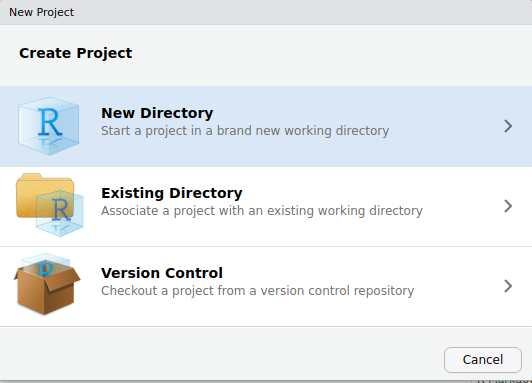
\includegraphics{images/installing_intro/newproj1.png}
  \item
    Click New Project:\\
    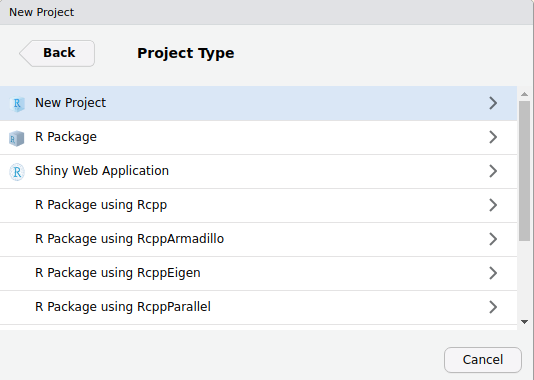
\includegraphics{images/installing_intro/newproj2.png}
  \item
    Name the project, and decide where you want to save it on your computer by clicking on browse. Then click Create Project:\\
    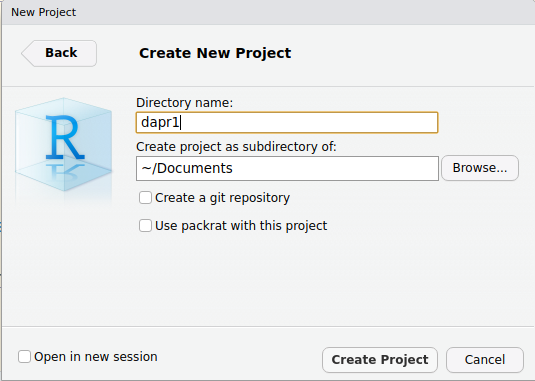
\includegraphics{images/installing_intro/newproj3.png}
  \end{itemize}
\end{enumerate}

\textbf{Option B: Rstudio Cloud (for chromebook users)}

\begin{enumerate}
\def\labelenumi{\arabic{enumi}.}
\tightlist
\item
  Register for Rstudio Cloud \href{https://rstudio.cloud/}{(https://rstudio.cloud/)}.
\item
  Log in to Rstudio Cloud
\item
  Create a new project
  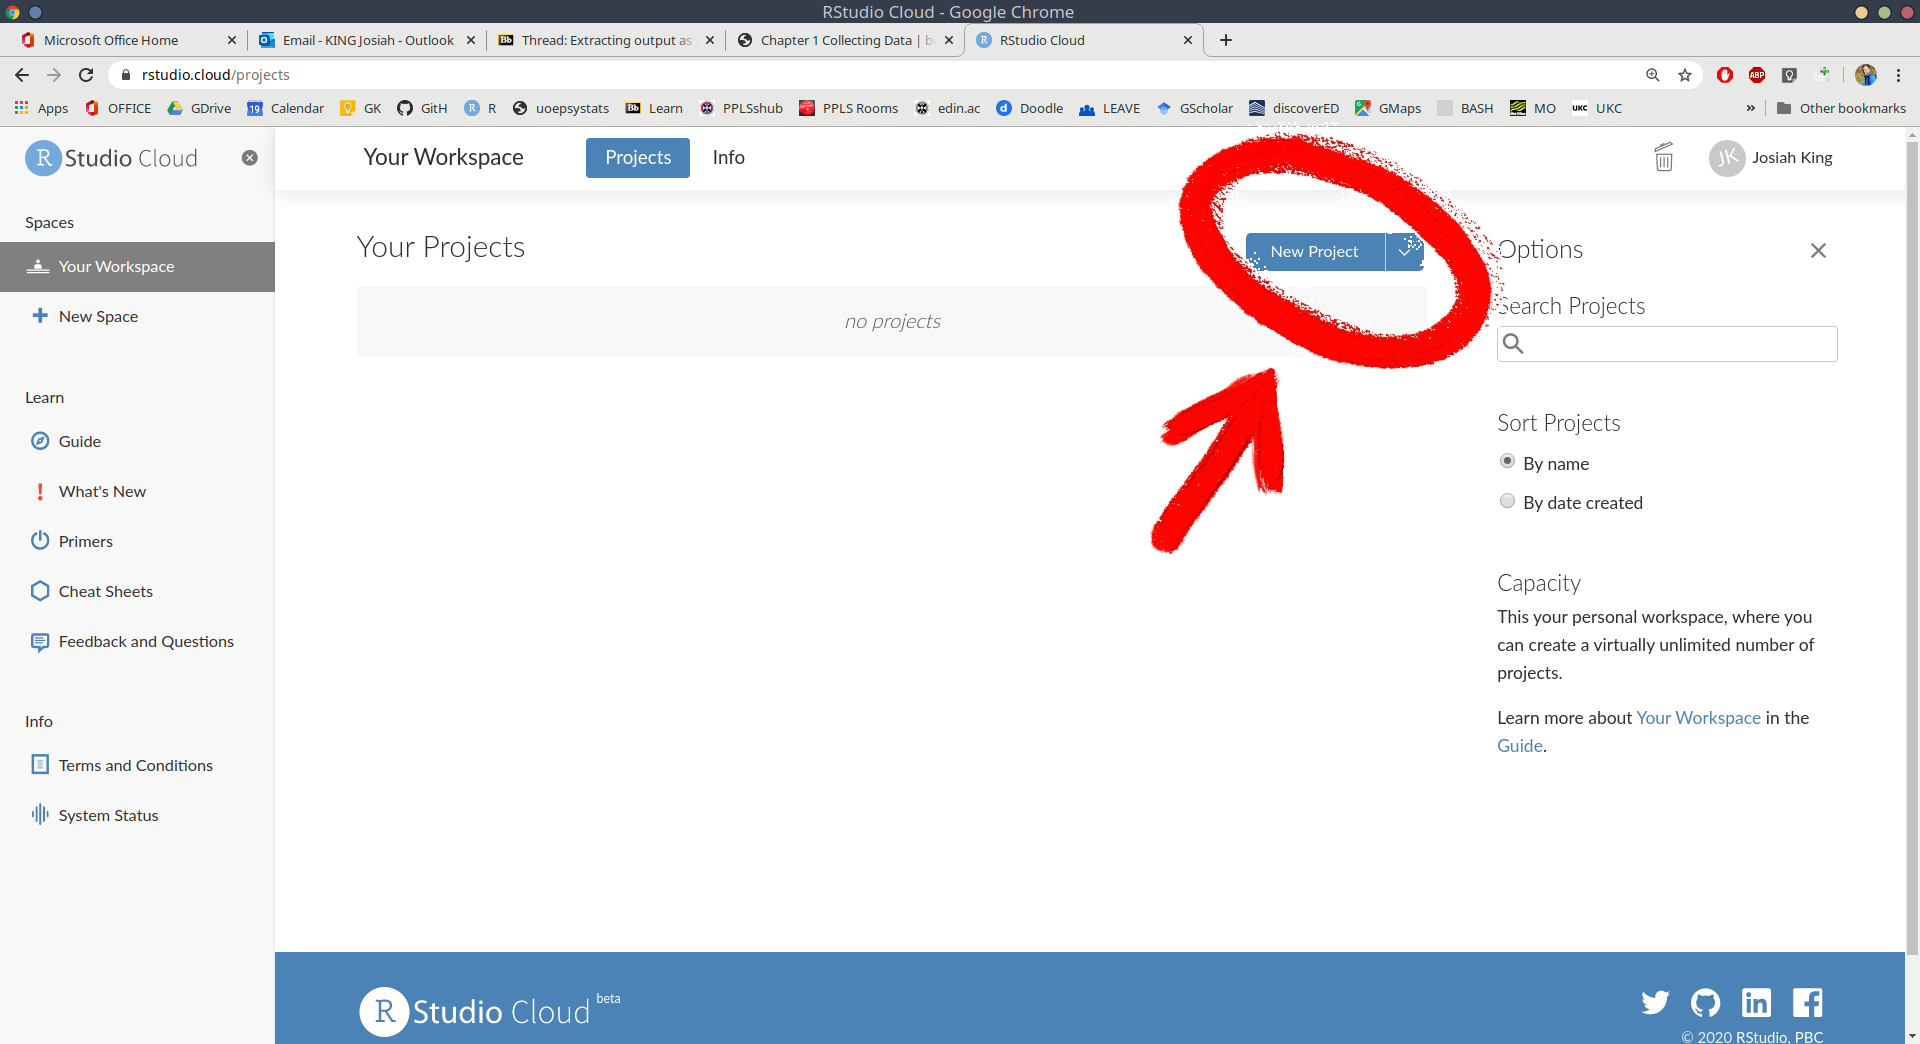
\includegraphics{images/installing_intro/rstudiocloud.png}
\item
  Rename the project
  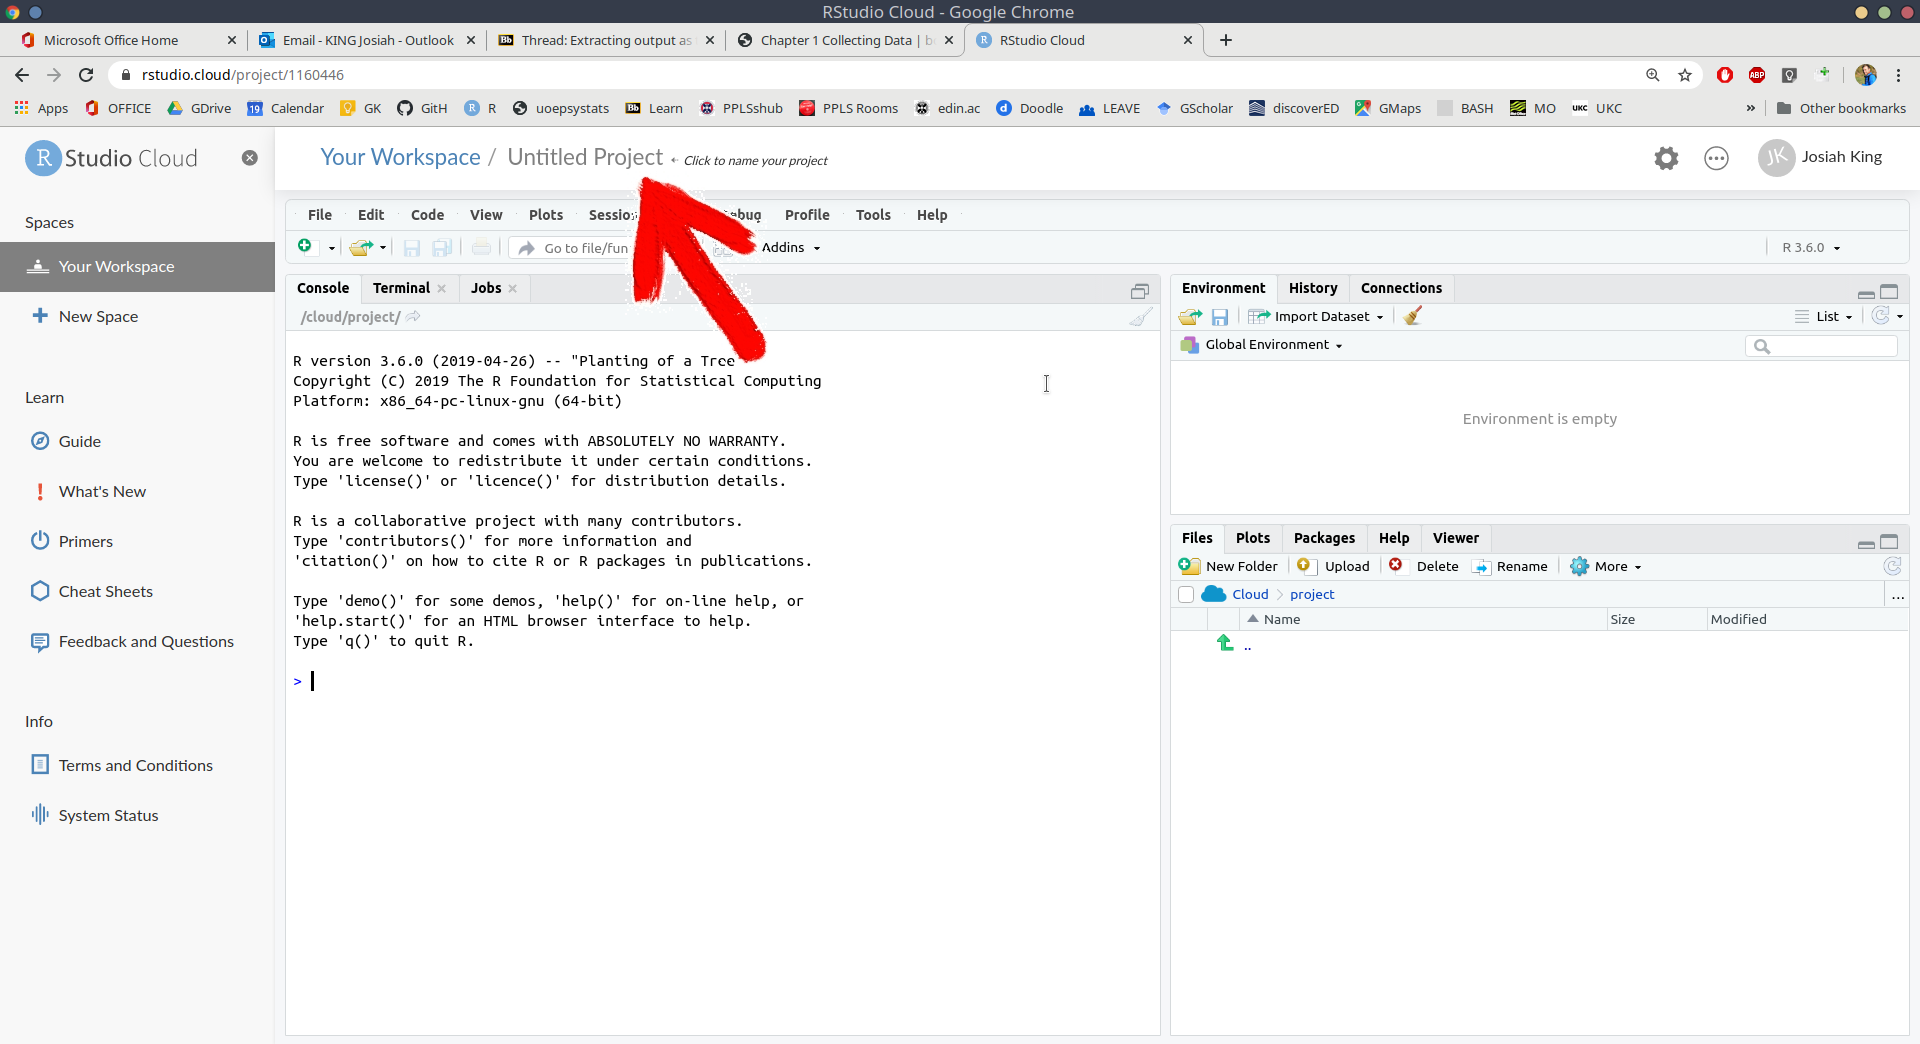
\includegraphics{images/installing_intro/rstudiocloud2.png}
\end{enumerate}

\hypertarget{first-look-at-rstudio}{%
\subsection*{First look at Rstudio}\label{first-look-at-rstudio}}
\addcontentsline{toc}{subsection}{First look at Rstudio}

Okay, now you should have a project open, and you should see something which looks more or less like the below, where there are several little windows.

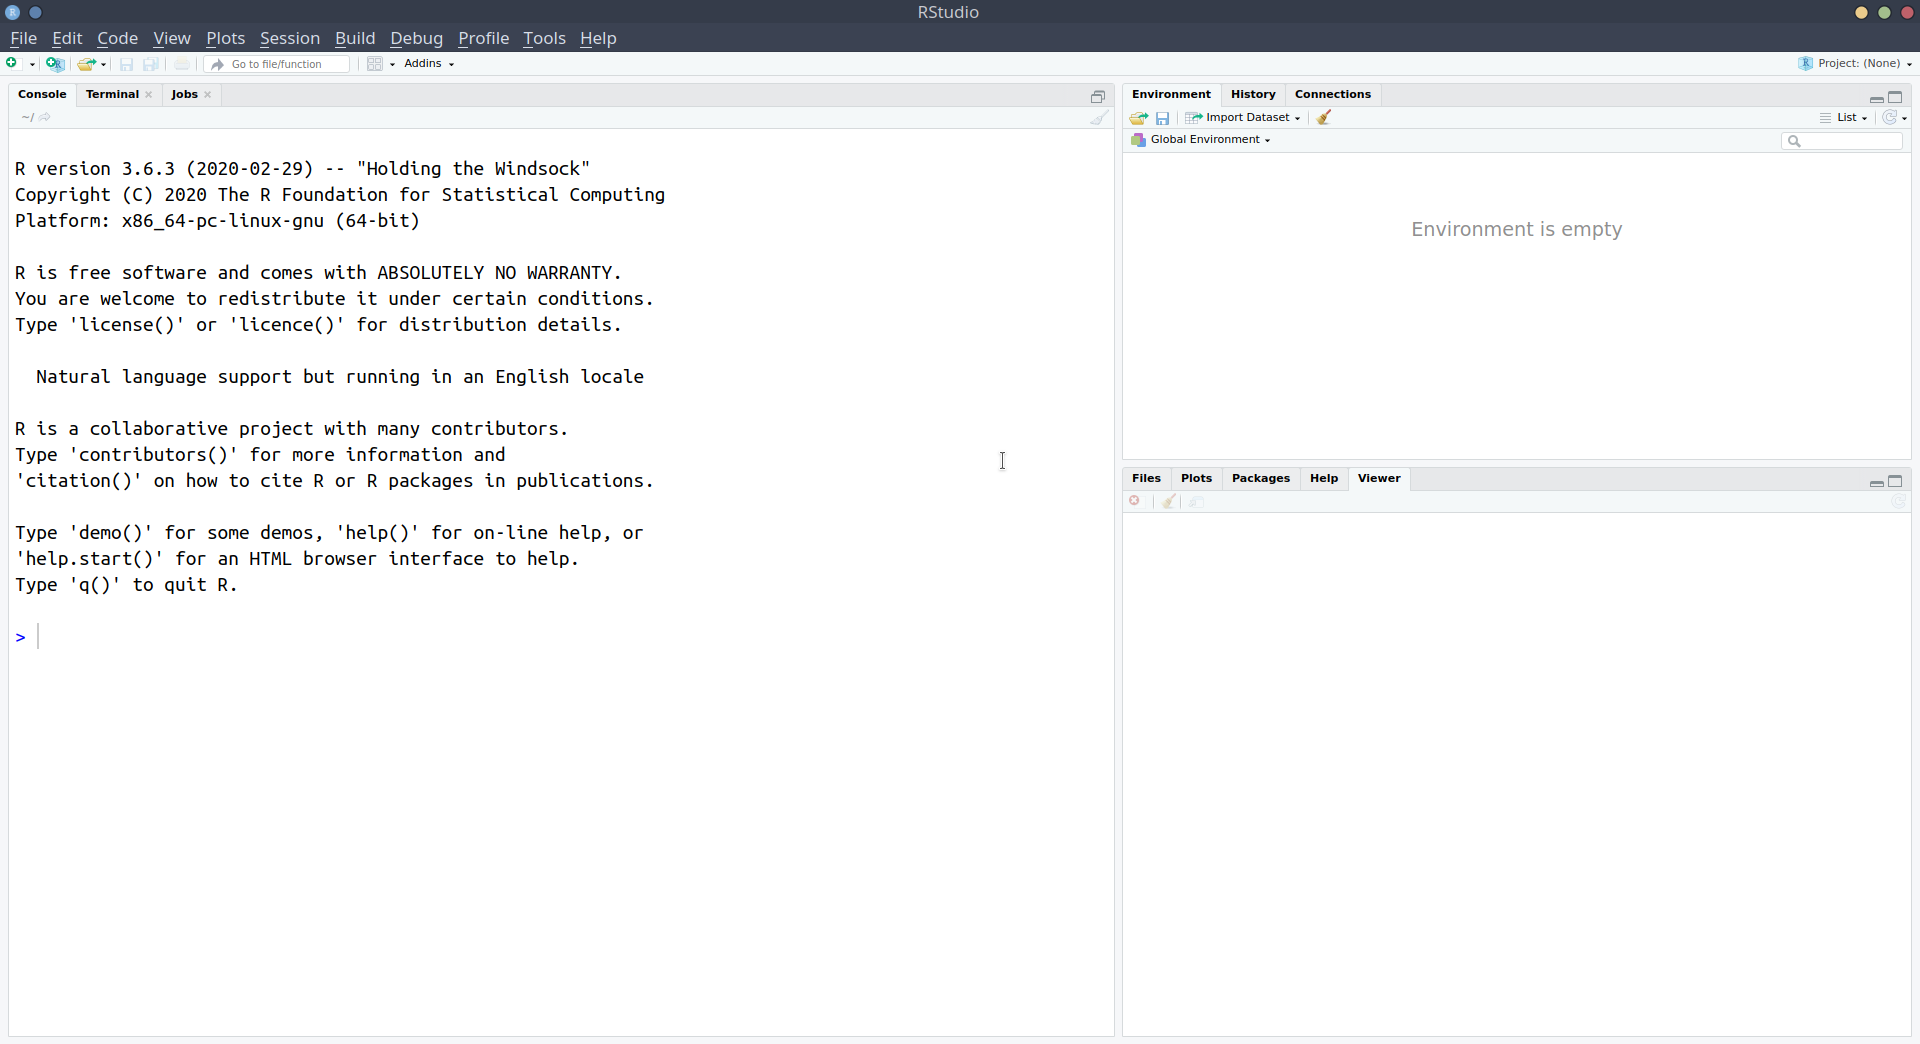
\includegraphics{images/installing_intro/freshr.png}

We're going to explore what each of these little windows offer by just diving in and starting to do things.

\hypertarget{r-as-a-calculator}{%
\subsection*{R as a calculator}\label{r-as-a-calculator}}
\addcontentsline{toc}{subsection}{R as a calculator}

Starting in the left-hand window, you'll notice the little blue arrow {\textgreater{}}.
This is where we R code gets \emph{executed}.
Type 2+2, and hit enter ↵

It's a calculator!

Let's work through some of the basic operations (adding, subtracting etc).\\
Try these commands yourself:

\begin{itemize}
\tightlist
\item
  \texttt{2+5}
\item
  \texttt{10-4}
\item
  \texttt{2*5}
\item
  \texttt{10-(2*5)}
\item
  \texttt{(10-2)*5}
\item
  \texttt{10/2}
\item
  \texttt{3\^{}2} (Hint, interpret the \texttt{\^{}} symbol as ``to the power of'')
\end{itemize}

\textbf{Helpful tip}

Whenever you see the blue arrow ({\textgreater{}}), it means R is ready and waiting for a command.

If you type \texttt{10+} and press enter, you'll see that instead of {\textgreater{}} you are left with {+}. This means that R is waiting for more. Either give it more, or cancel the command by pressing the escape key on your keyboard.

Now let's take a sidestep.\\
As well as performing calculations, we can \emph{ask} R things, such as ``Is 3 less than 5?'':

\begin{Shaded}
\begin{Highlighting}[]
\DecValTok{3}\OperatorTok{<}\DecValTok{5}
\end{Highlighting}
\end{Shaded}

\begin{verbatim}
[1] TRUE
\end{verbatim}

Try the following:

\begin{itemize}
\tightlist
\item
  \texttt{3\textgreater{}5} - ``is 3 greater than 5?''
\item
  \texttt{3\textless{}=5} - ``is 3 less than OR equal to 5?''
\item
  \texttt{3\textgreater{}=3} - ``is 3 greater than OR equal to 3?''
\item
  \texttt{3==5} - ``is 3 equal to 5?''
\item
  \texttt{(2*5)==10} ``is 2 times 5 equal to 10?''
\item
  \texttt{(2*5)!=11} ``is 2 times 5 NOT equal to 11?''
\end{itemize}

\hypertarget{r-as-a-calculator-with-a-memory}{%
\subsection*{R as a calculator with a memory}\label{r-as-a-calculator-with-a-memory}}
\addcontentsline{toc}{subsection}{R as a calculator with a memory}

We can also store things in R's memory, and to that we just need to give them a name.\\
Type \texttt{x\ \textless{}-\ 5} and press enter.

What has happened? We've just stored something named \texttt{x} which has the value \texttt{5}.
We can now refer to the name and it will give us the value!
Try typing \texttt{x} and hitting enter. It should give you the number 5.\\
What about \texttt{x*3}?

\textbf{Storing things in R}

The \texttt{\textless{}-} symbol is used to \emph{assign} a value to a named object.

\emph{{[}name{]}} \textless{}- \emph{{[}value{]}}

Note, there are a few rules about names in R:

\begin{itemize}
\tightlist
\item
  No spaces - spaces \emph{inside} a name are not allowed (the spaces around the \texttt{\textless{}-} don't matter):

  \begin{itemize}
  \tightlist
  \item
    \texttt{lucky\_number\ \textless{}-\ 5} ✔   \texttt{lucky\ number\ \textless{}-\ 5} ❌\\
  \end{itemize}
\item
  Names must start with a letter:

  \begin{itemize}
  \tightlist
  \item
    \texttt{lucky\_number\ \textless{}-\ 5} ✔   \texttt{1lucky\_number\ \textless{}-\ 5} ❌\\
  \end{itemize}
\item
  Case sensitive:

  \begin{itemize}
  \tightlist
  \item
    \texttt{lucky\_number} is different from \texttt{Lucky\_Number}\\
  \end{itemize}
\item
  Reserved words - there is a set of words you can't use as names, including: if, else, for, in, TRUE, FALSE, NULL, NA, NaN, function\\
  (Don't worry about remembering these, R will tell you if you make the mistake of trying to name a variable after one of these).
\end{itemize}

You might have noticed that something else happened when you executed the code \texttt{x\textless{}-5}.
The thing we named \textbf{x} with a value of \textbf{5} suddenly appeared in the top-right window. This is known as the \textbf{environment}, and it shows everything that we store things in R:

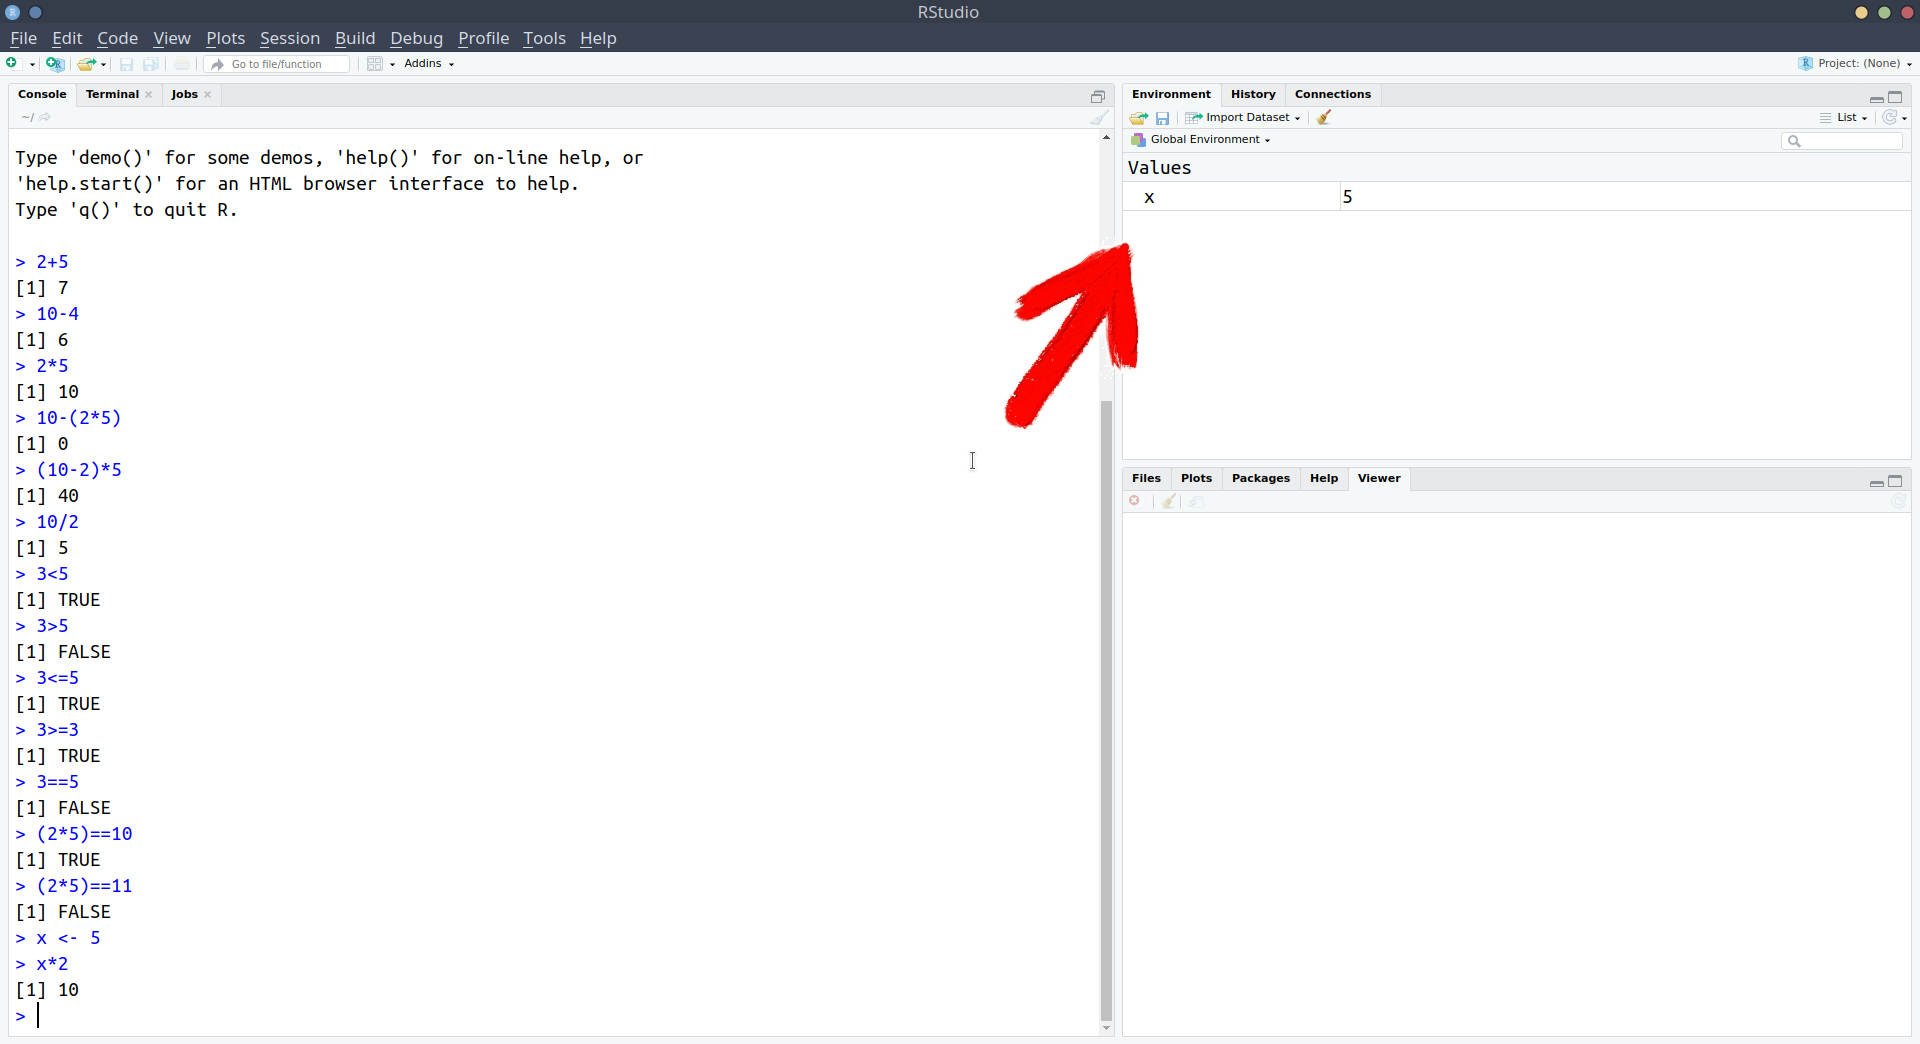
\includegraphics{images/installing_intro/rassign.png}

We've now used a couple of the windows - we've been executing R code in the \textbf{console}, and learned about how we can store things in R's memory (the \textbf{environment}) by assigning a name to them:

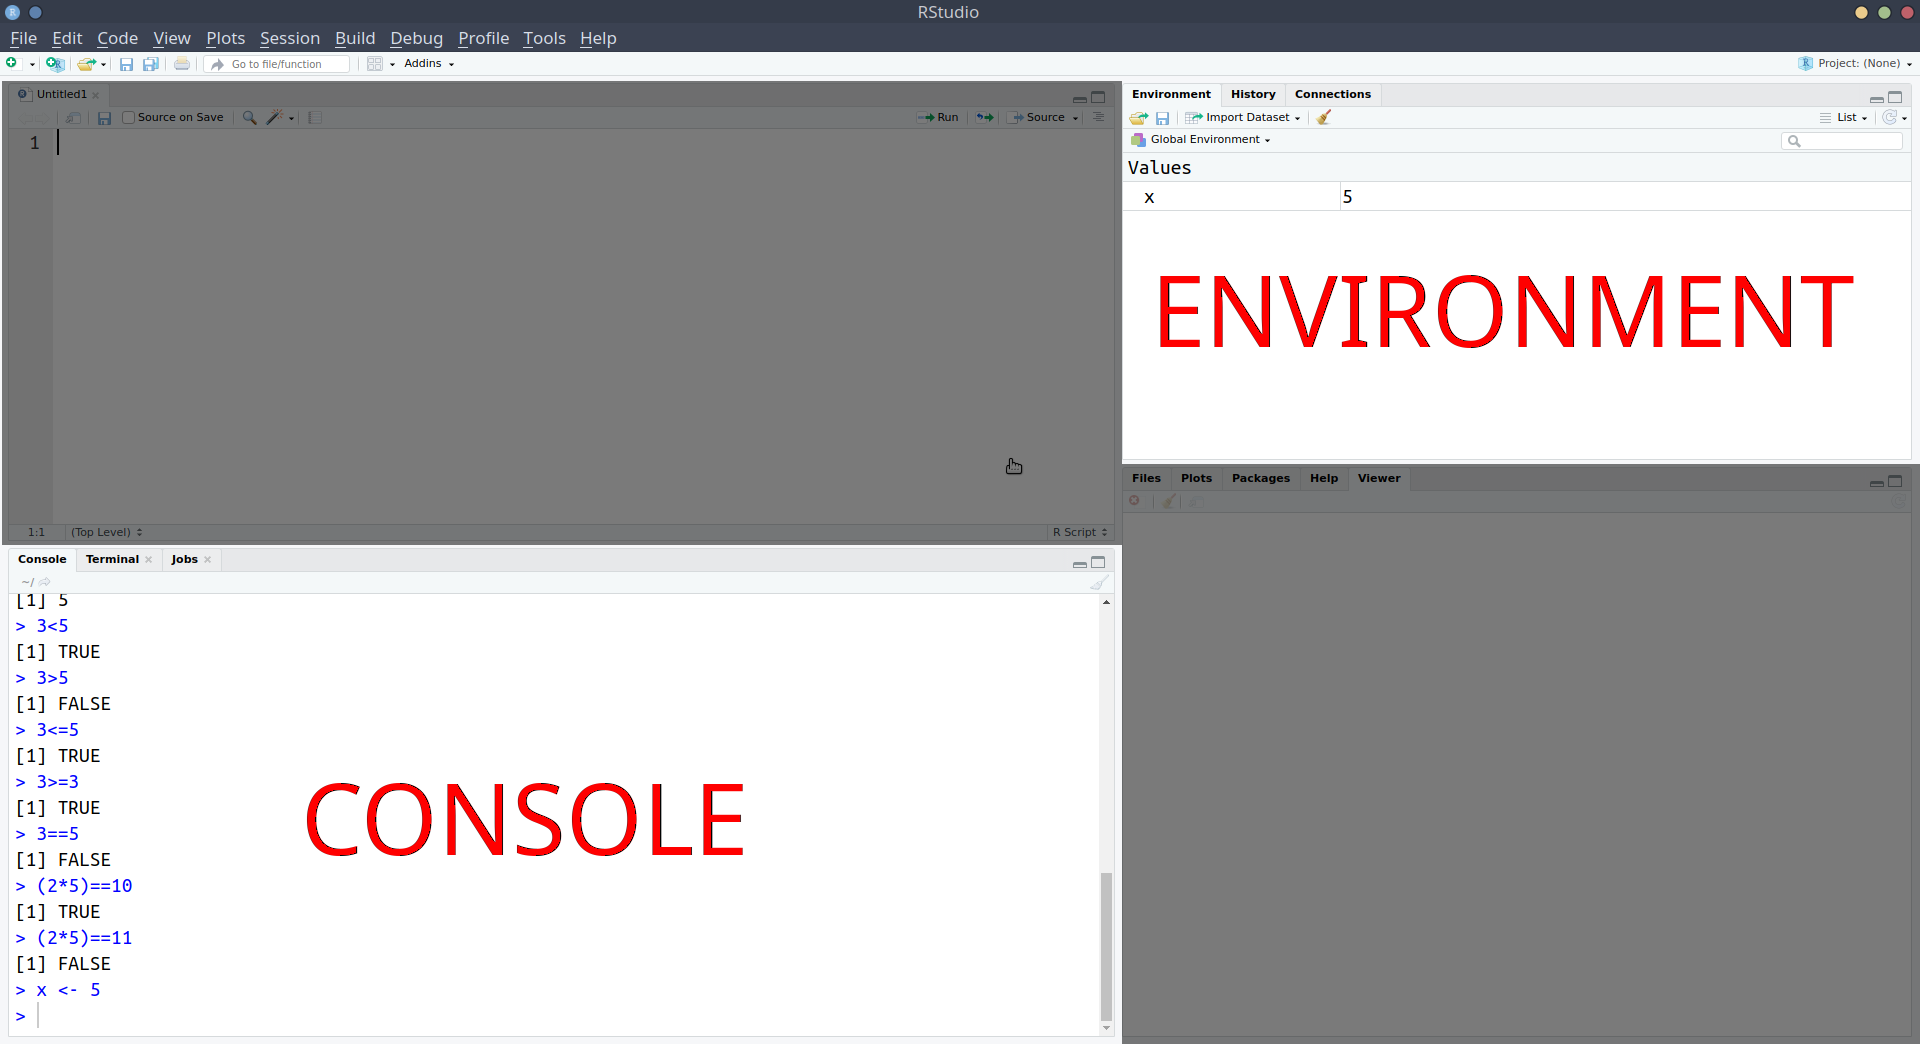
\includegraphics{images/installing_intro/r4panel2.png}

Notice that in the screenshot above, we have moved the \textbf{console} down to the bottom-left, and introduced a new window above it. This is the one that we're going to talk about next.

\hypertarget{rscripts-and-rmarkdown}{%
\subsection*{Rscripts and Rmarkdown}\label{rscripts-and-rmarkdown}}
\addcontentsline{toc}{subsection}{Rscripts and Rmarkdown}

What if we want to edit our code?\\
Whatever we write in the console just disappears upwards. What if we want to change things we did earlier on?

Well, we can write and edit our code in a separate place \emph{before} sending it to the \textbf{console} to be executed!!

\hypertarget{r-scripts}{%
\subsubsection*{R scripts}\label{r-scripts}}
\addcontentsline{toc}{subsubsection}{R scripts}

\textbf{Task}
1. Open an R script
+ \textbf{File \textgreater{} New File \textgreater{} R script}
1. Copy and paste the following into the R script

\begin{Shaded}
\begin{Highlighting}[]
\NormalTok{x<-}\DecValTok{210}
\NormalTok{y<-}\DecValTok{15}
\NormalTok{x}\OperatorTok{/}\NormalTok{y}
\end{Highlighting}
\end{Shaded}

\begin{enumerate}
\def\labelenumi{\arabic{enumi}.}
\tightlist
\item
  With your text-cursor (blinking vertical line) on the top line:

  \begin{itemize}
  \tightlist
  \item
    Ctrl + enter (Windows)
  \item
    Cmd + enter (MacOS)
  \end{itemize}
\end{enumerate}

Notice what has happened - it has sent the command \texttt{x\textless{}-210} to the console, where it has been executed, and \textbf{x} is now in your environment.\\
Additionally, it has moved the text-cursor to the next line.\\
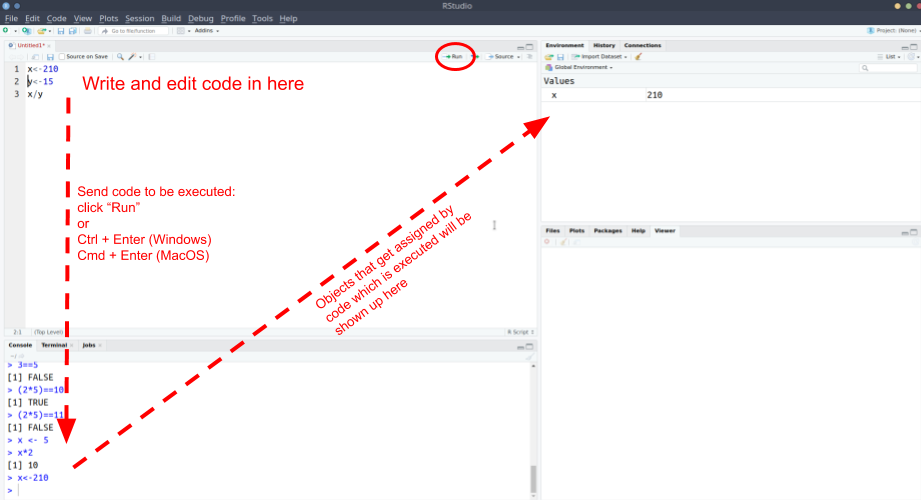
\includegraphics{images/installing_intro/reditor.png}

\textbf{Task}
Press Ctrl + enter (Windows) or Cmd + enter (MacOS) again.\\
Do it twice (this will run the next two lines).

Then, change \textbf{x} to some other number in your R script, and run the lines again (starting at the top).

\textbf{Task}
Add the following line to your Rscript and execute it (send it to the console pressing Ctrl/Cmd + Enter):

\begin{Shaded}
\begin{Highlighting}[]
\KeywordTok{plot}\NormalTok{(}\DecValTok{1}\NormalTok{,}\DecValTok{5}\NormalTok{)}
\end{Highlighting}
\end{Shaded}

A very basic plot should have appeared in the bottom-right of Rstudio.
The bottom-right window actually does some other useful things.

\textbf{Task}
1. Save the Rscript you have been working with:
+ File \textgreater{} Save
+ give it an appropriate name, and click save.
1. Check that you can now see that file in the project, by clicking on the ``Files'' tab of the bottom-right window.

\hypertarget{rmarkdown}{%
\subsubsection*{Rmarkdown}\label{rmarkdown}}
\addcontentsline{toc}{subsubsection}{Rmarkdown}

In addition to R scripts, there is another type of document we can create, known as an ``Rmarkdown''.

Rmarkdown documents combine the analytical power of R and the utility of a text-processor.
We can have one document which contains all of our analysis as well as our written text, and can be \emph{compiled} into a nicely formatted report. This saves us doing analysis in R and copying results across to Microsoft Word. It ensures our report accurately reflects our analysis. Everything that you're reading now has all been written in Rmarkdown!

We're going to use Rmarkdown documents throughout this course. We'll get into it how to write them lower down, but it basically involves writing normal text interspersed with ``code-chunks'' (i.e., chunks of code!).\\
In the example below, you can see the grey boxes indicating the R code, with text in between.\\
We can then compile the document into either a \textbf{.pdf} or a \textbf{.html}.

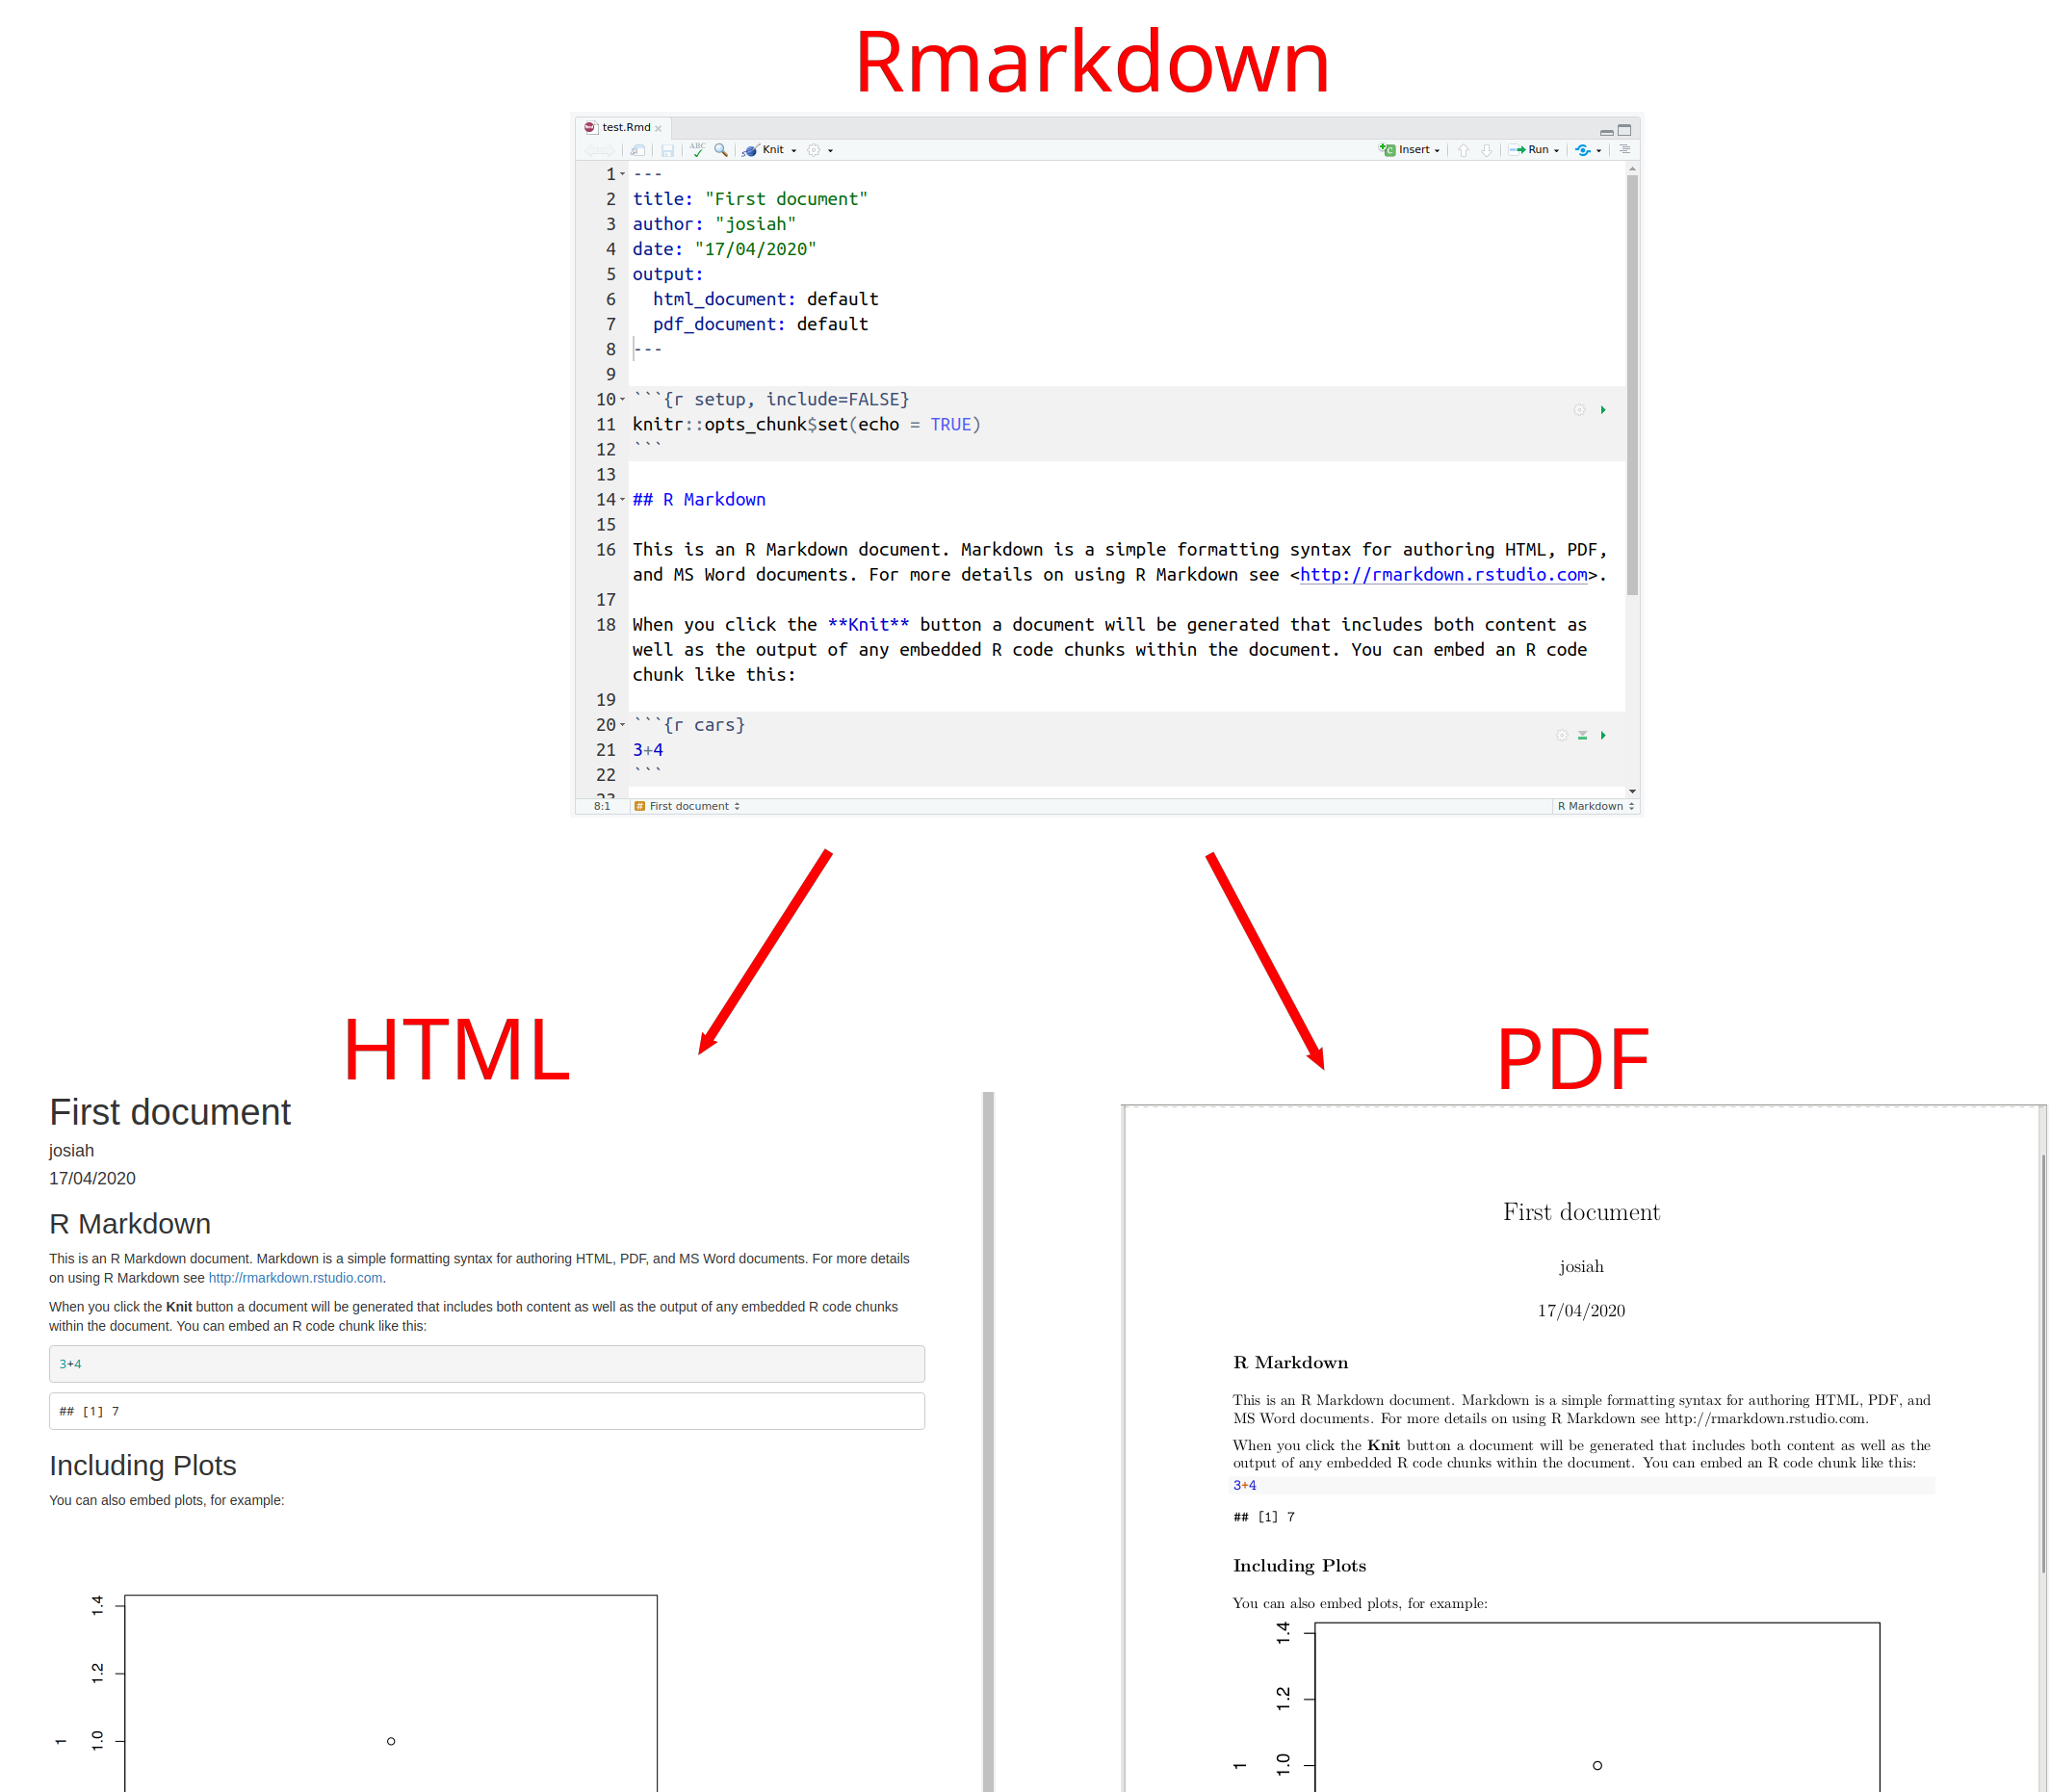
\includegraphics{images/installing_intro/compiling.png}

\hypertarget{recap}{%
\subsection*{Recap}\label{recap}}
\addcontentsline{toc}{subsection}{Recap}

Okay, so we've now seen all of the different windows in Rstudio in action:

\begin{itemize}
\tightlist
\item
  The \textbf{console} is where R code gets executed
\item
  The \textbf{environment} is R's memory, you can \emph{assign} something a name and store it here, and then refer to it by name in your code.
\item
  The \textbf{editor} is where you can write and edit R code and Rmarkdown documents. You can then send this to the console for it to be executed.
\item
  The bottom-right window shows you the \textbf{plots} that you create, the \textbf{files} in your project, and some other things (we'll get to these later).
\end{itemize}

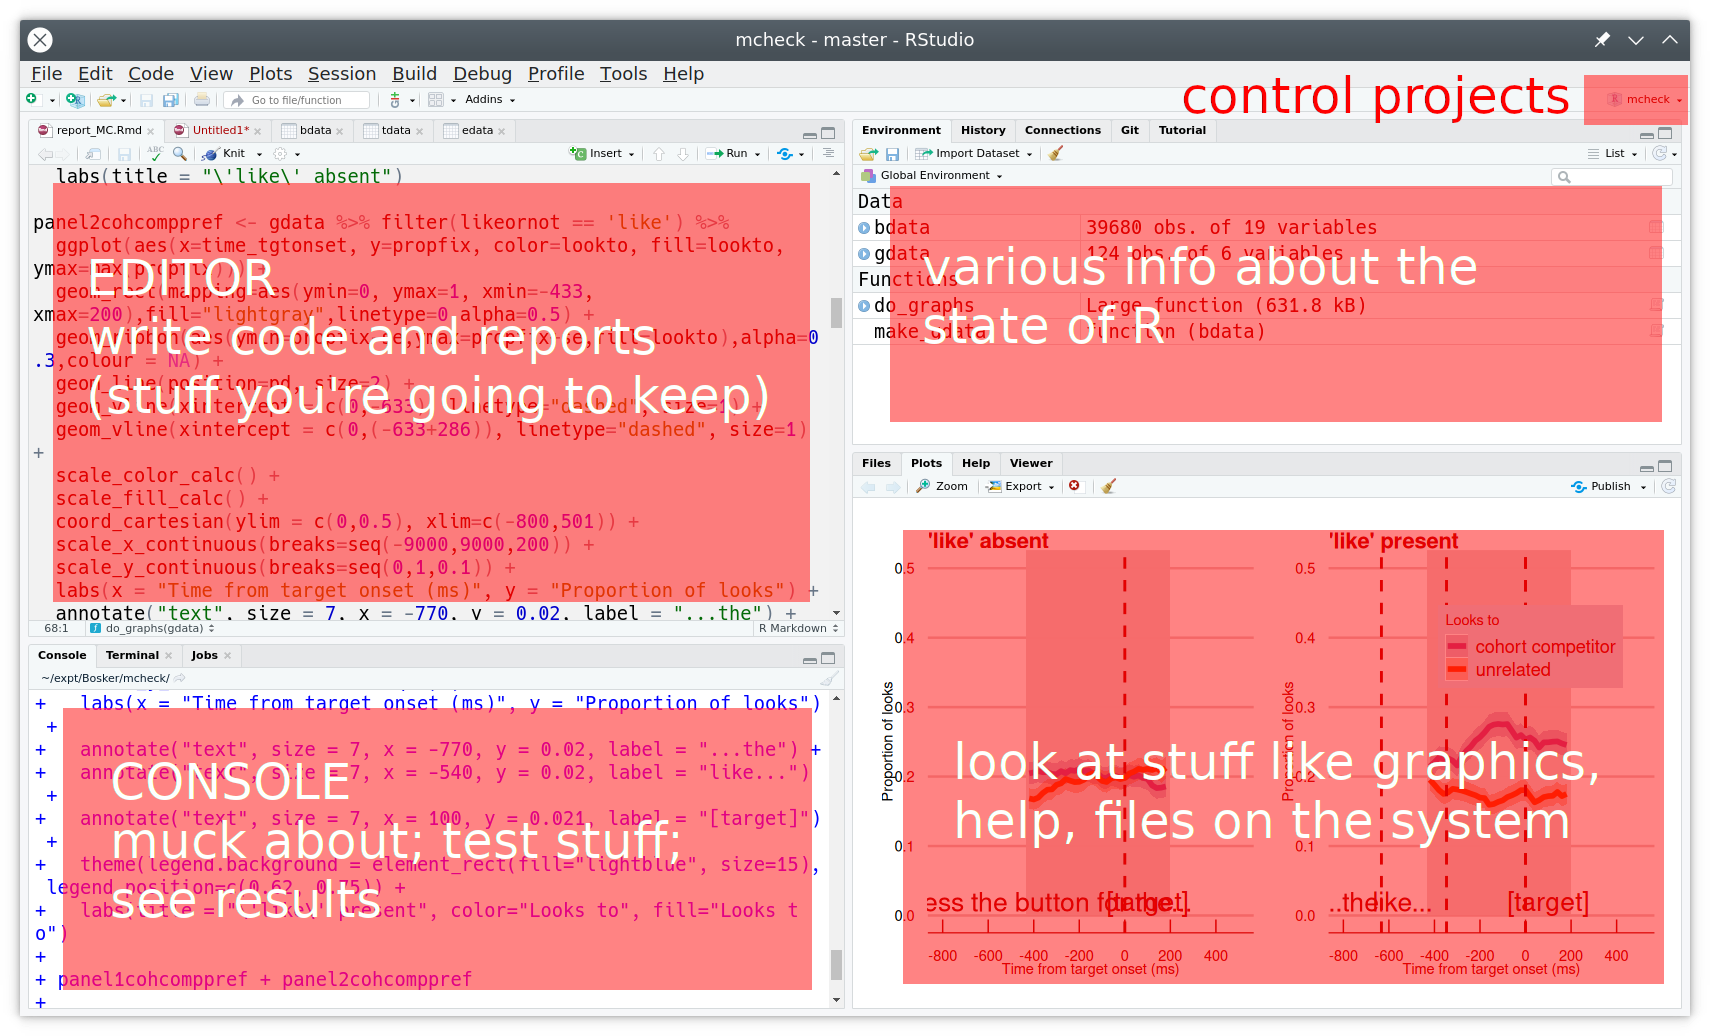
\includegraphics{images/installing_intro/r4panel3.png}

\begin{center}\rule{0.5\linewidth}{0.5pt}\end{center}

\hypertarget{take-a-breather}{%
\section{Take a breather}\label{take-a-breather}}

Below are a couple of our recommended settings for you to change as you begin your journey in R.
After you've changed them, take a 5 minute break before moving on to learning about how we store data in R.

\textbf{Useful Settings 1: Clean environments}

As you use R more, you will store lots of things with different names. Throughout this course alone, you'll probably name hundreds of different things.\\
This could quickly get messy within our project.

We can make it so that we have a clean environment each time you open Rstudio. This will be really handy.

\begin{enumerate}
\def\labelenumi{\arabic{enumi}.}
\tightlist
\item
  In the top menu, click\\
  \textbf{Tools \textgreater{} Global Options\ldots{}}
\item
  Then, \emph{untick} the box for ``Restore .RData into workspace at startup'', and change ``Save workspace to .RData on exit'' to ``Never'':
  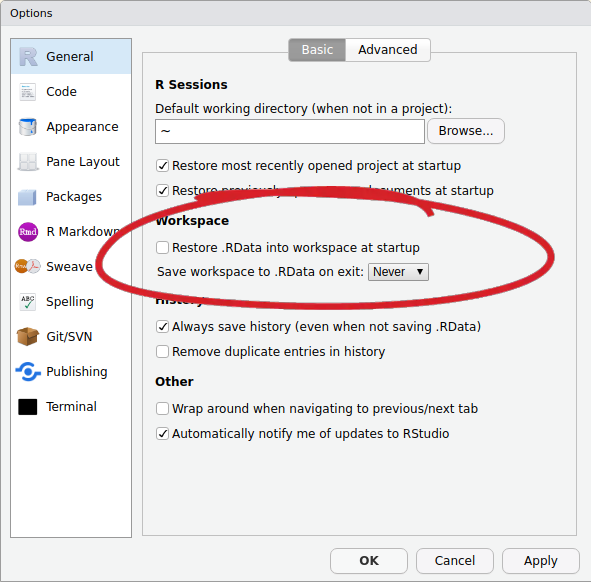
\includegraphics{images/installing_intro/renvsettings.png}
\end{enumerate}

\textbf{Useful Settings 2: Wrapping code}

In the editor, you might end up with a line of code which is really long:

\begin{Shaded}
\begin{Highlighting}[]
\NormalTok{x <-}\StringTok{ }\DecValTok{1}\OperatorTok{+}\DecValTok{2}\OperatorTok{+}\DecValTok{3}\OperatorTok{+}\DecValTok{6}\OperatorTok{+}\DecValTok{3}\OperatorTok{+}\DecValTok{45}\OperatorTok{+}\DecValTok{8467}\OperatorTok{+}\DecValTok{356}\OperatorTok{+}\DecValTok{8565}\OperatorTok{+}\DecValTok{34}\OperatorTok{+}\DecValTok{34}\OperatorTok{+}\DecValTok{657}\OperatorTok{+}\DecValTok{6756}\OperatorTok{+}\DecValTok{456}\OperatorTok{+}\DecValTok{456}\OperatorTok{+}\DecValTok{54}\OperatorTok{+}\DecValTok{3}\OperatorTok{+}\DecValTok{78}\OperatorTok{+}\DecValTok{3}\OperatorTok{+}\DecValTok{3476}\OperatorTok{+}\DecValTok{8}\OperatorTok{+}\DecValTok{4}\OperatorTok{+}\DecValTok{67}\OperatorTok{+}\DecValTok{456}\OperatorTok{+}\DecValTok{567}\OperatorTok{+}\DecValTok{3}\OperatorTok{+}\DecValTok{34575}\OperatorTok{+}\DecValTok{45}\OperatorTok{+}\DecValTok{2}\OperatorTok{+}\DecValTok{6}\OperatorTok{+}\DecValTok{9}\OperatorTok{+}\DecValTok{5}\OperatorTok{+}\DecValTok{6}
\end{Highlighting}
\end{Shaded}

You can make Rstudio `wrap' the line, so that you can see it all, without having to scroll.

\begin{Shaded}
\begin{Highlighting}[]
\NormalTok{x <-}\StringTok{ }\DecValTok{1}\OperatorTok{+}\DecValTok{2}\OperatorTok{+}\DecValTok{3}\OperatorTok{+}\DecValTok{6}\OperatorTok{+}\DecValTok{3}\OperatorTok{+}\DecValTok{45}\OperatorTok{+}\DecValTok{8467}\OperatorTok{+}\DecValTok{356}\OperatorTok{+}\DecValTok{8565}\OperatorTok{+}\DecValTok{34}\OperatorTok{+}\DecValTok{34}\OperatorTok{+}\DecValTok{657}\OperatorTok{+}\DecValTok{6756}\OperatorTok{+}\DecValTok{456}\OperatorTok{+}\DecValTok{456}\OperatorTok{+}\DecValTok{54}\OperatorTok{+}\DecValTok{3}\OperatorTok{+}\DecValTok{78}\OperatorTok{+}\DecValTok{3}\OperatorTok{+}\DecValTok{3476}\OperatorTok{+}\DecValTok{8}\OperatorTok{+}\DecValTok{4}\OperatorTok{+}\DecValTok{67}\OperatorTok{+}
\DecValTok{456}\OperatorTok{+}\DecValTok{567}\OperatorTok{+}\DecValTok{3}\OperatorTok{+}\DecValTok{34575}\OperatorTok{+}\DecValTok{45}\OperatorTok{+}\DecValTok{2}\OperatorTok{+}\DecValTok{6}\OperatorTok{+}\DecValTok{9}\OperatorTok{+}\DecValTok{5}\OperatorTok{+}\DecValTok{6}
\end{Highlighting}
\end{Shaded}

\begin{enumerate}
\def\labelenumi{\arabic{enumi}.}
\tightlist
\item
  In the top menu, click\\
  \textbf{Tools \textgreater{} Global Options\ldots{}}
\item
  In the left menu of the box, click ``Code''
\item
  \emph{Tick} the box for ``Soft-wrap R source files''
\end{enumerate}

\begin{center}\rule{0.5\linewidth}{0.5pt}\end{center}

\hypertarget{data-in-r}{%
\section{Data in R}\label{data-in-r}}

\hypertarget{installing-r-packages}{%
\subsection*{Installing R packages}\label{installing-r-packages}}
\addcontentsline{toc}{subsection}{Installing R packages}

Alongside the basic installation of R and Rstudio, there are many add-on packages which the R community create and maintain.

The thousands of packages are part of what makes R such a powerful and useful tool - there is a package for almost everything you could want to do in R.

In order to be able to write and compile Rmarkdown documents (and do a whole load of other things which we are going to need throughout the course) we are now going to install a set of packages known collectively as the ``tidyverse''.

\textbf{Task}
In the \textbf{console}, type \texttt{install.packages("tidyverse")} and hit enter.

Lots of red text will come up, and it will take a bit of time.

When it has finished, and R is ready for you to use again, you will see the little blue arrow {\textgreater{}}.

\hypertarget{starting-a-new-.rmd-document}{%
\subsection*{Starting a new .Rmd document}\label{starting-a-new-.rmd-document}}
\addcontentsline{toc}{subsection}{Starting a new .Rmd document}

\textbf{Task}
Open a new Rmarkdown document.

\textbf{File \textgreater{} New File \textgreater{} R Markdown..}

When the box pops-up, give a title of your choice (``Intro lab'', maybe?) and your name as the author.

The file which opens will have some template stuff in it. Delete everything below the first code chunk to start with a fresh document:

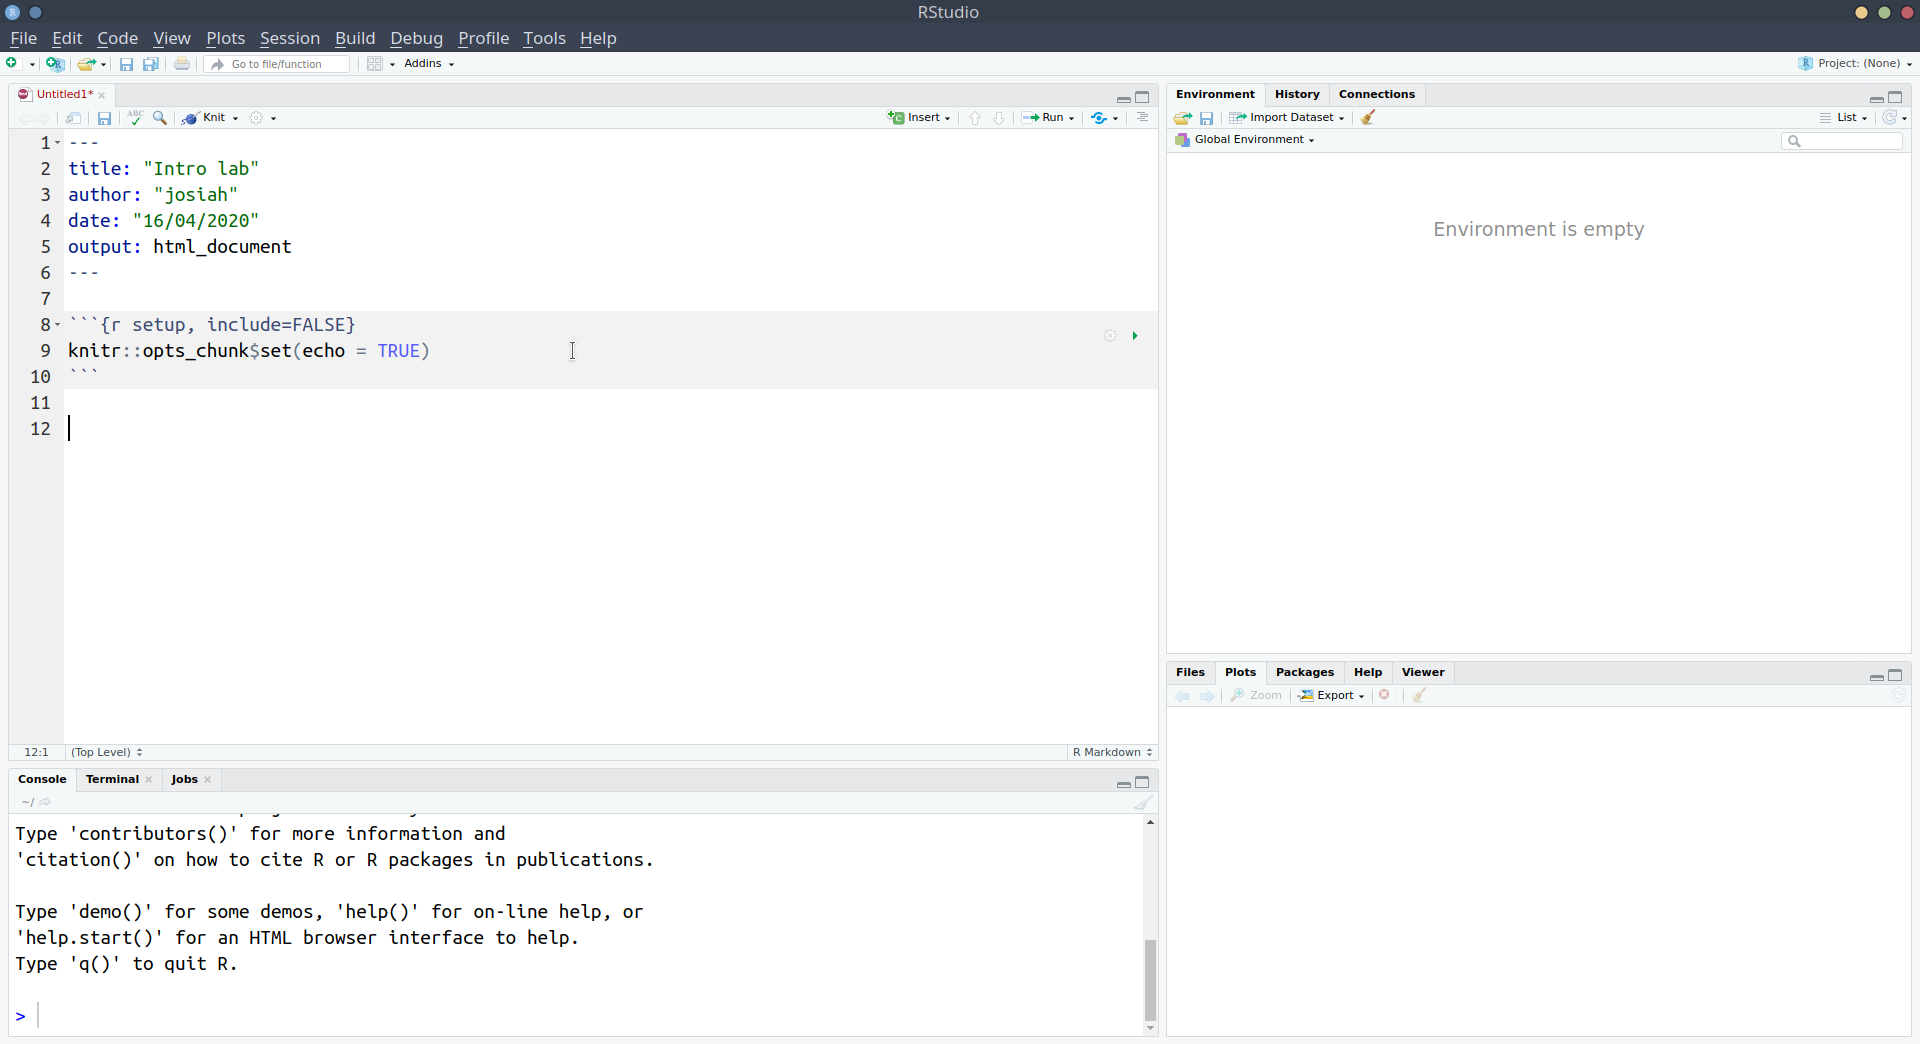
\includegraphics{images/installing_intro/ss_newrmd.png}

\textbf{Task}
Insert a new code chunk by either using the Insert button in the top right of the document, and clicking R, or typing \emph{Ctrl + Alt + i}

Inside the chunk, type:\\
\texttt{print("Hello\ world!\ My\ name\ is\ ?")}.

To execute the code inside the chunk, you can either:

\begin{itemize}
\tightlist
\item
  do as you did in the R script - put the text-cursor on the first line, and hit Ctrl/Cmd + Enter to run the lines sequentially
\item
  click the little green arrow at the top right of your code-chunk to run all of the code inside the chunk.
\end{itemize}

You can see that the output gets printed below.

\hypertarget{using-r-packages}{%
\subsection*{Using R packages}\label{using-r-packages}}
\addcontentsline{toc}{subsection}{Using R packages}

We're going to use some functions which are in the \textbf{tidyverse} package, which already installed above.\\
However, it's not enough just to install it - to actually \emph{use} the package, we need to load it using \texttt{library(tidyverse)}.

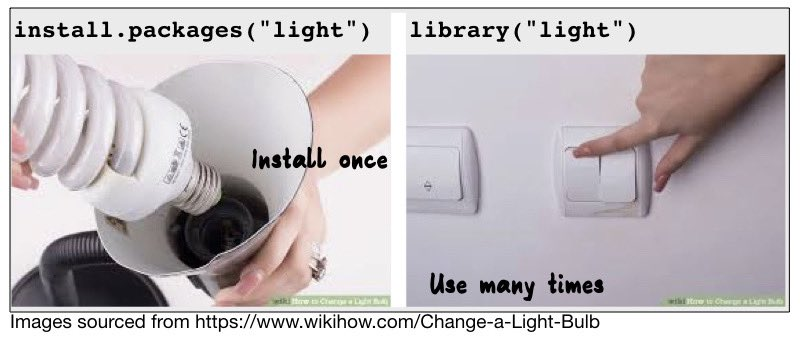
\includegraphics{images/installing_intro/libraries.jpeg}
(source: \url{https://twitter.com/visnut/status/1248087845589274624})

When writing analysis code, we want it to be \textbf{reproducible} - we want to be able to give somebody else our code and the data, and ensure that they can get the same results. To do this, we need to show what packages we use.\\
It is good practice to load any packages you use at the top of your code.

\textbf{Task}
In your first code chunk, type:

\begin{Shaded}
\begin{Highlighting}[]
\CommentTok{#I'm going to use these packages in this document:}
\KeywordTok{library}\NormalTok{(tidyverse)}
\end{Highlighting}
\end{Shaded}

and run the chunk.\\
\emph{Note, you might get various messages popping up below when you run this chunk, that is fine).}\\
:::yellow\\
\textbf{Comments in code}\\
Note that using \texttt{\#} in R code makes that line a comment, which basically means that R will ignore the line. Comments are useful for you to remind yourself of what your code is doing.
:::

\textbf{Task}
\textbf{Below} the code chunk, add a new line with the following:

\# R code examples

Note that when the \# is used in a Rmarkdown file \textbf{outside} of a code-chunk, it will make that line a heading when we finally get to \emph{compiling} the document. Below, what you see on the left will be compiled to look like those on the right:\\
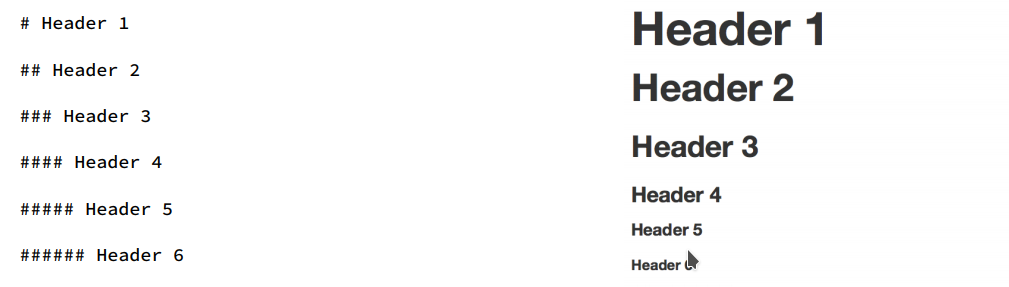
\includegraphics{images/installing_intro/headings.png}

\textbf{Task}
In your Rmarkdown document, choose a few of the symbols below, and write an explanation of what it does, giving an example in a code chunk. You can see an example of the first few below.

\begin{itemize}
\tightlist
\item
  \texttt{+}
\item
  \texttt{-}
\item
  \texttt{*}
\item
  \texttt{/}
\item
  \texttt{()}
\item
  \texttt{\^{}}
\item
  \texttt{\textless{}-}
\item
  \texttt{\textless{}}
\item
  \texttt{\textgreater{}}
\item
  \texttt{\textless{}=}
\item
  \texttt{\textgreater{}=}
\item
  \texttt{==}
\item
  \texttt{!=}
\end{itemize}

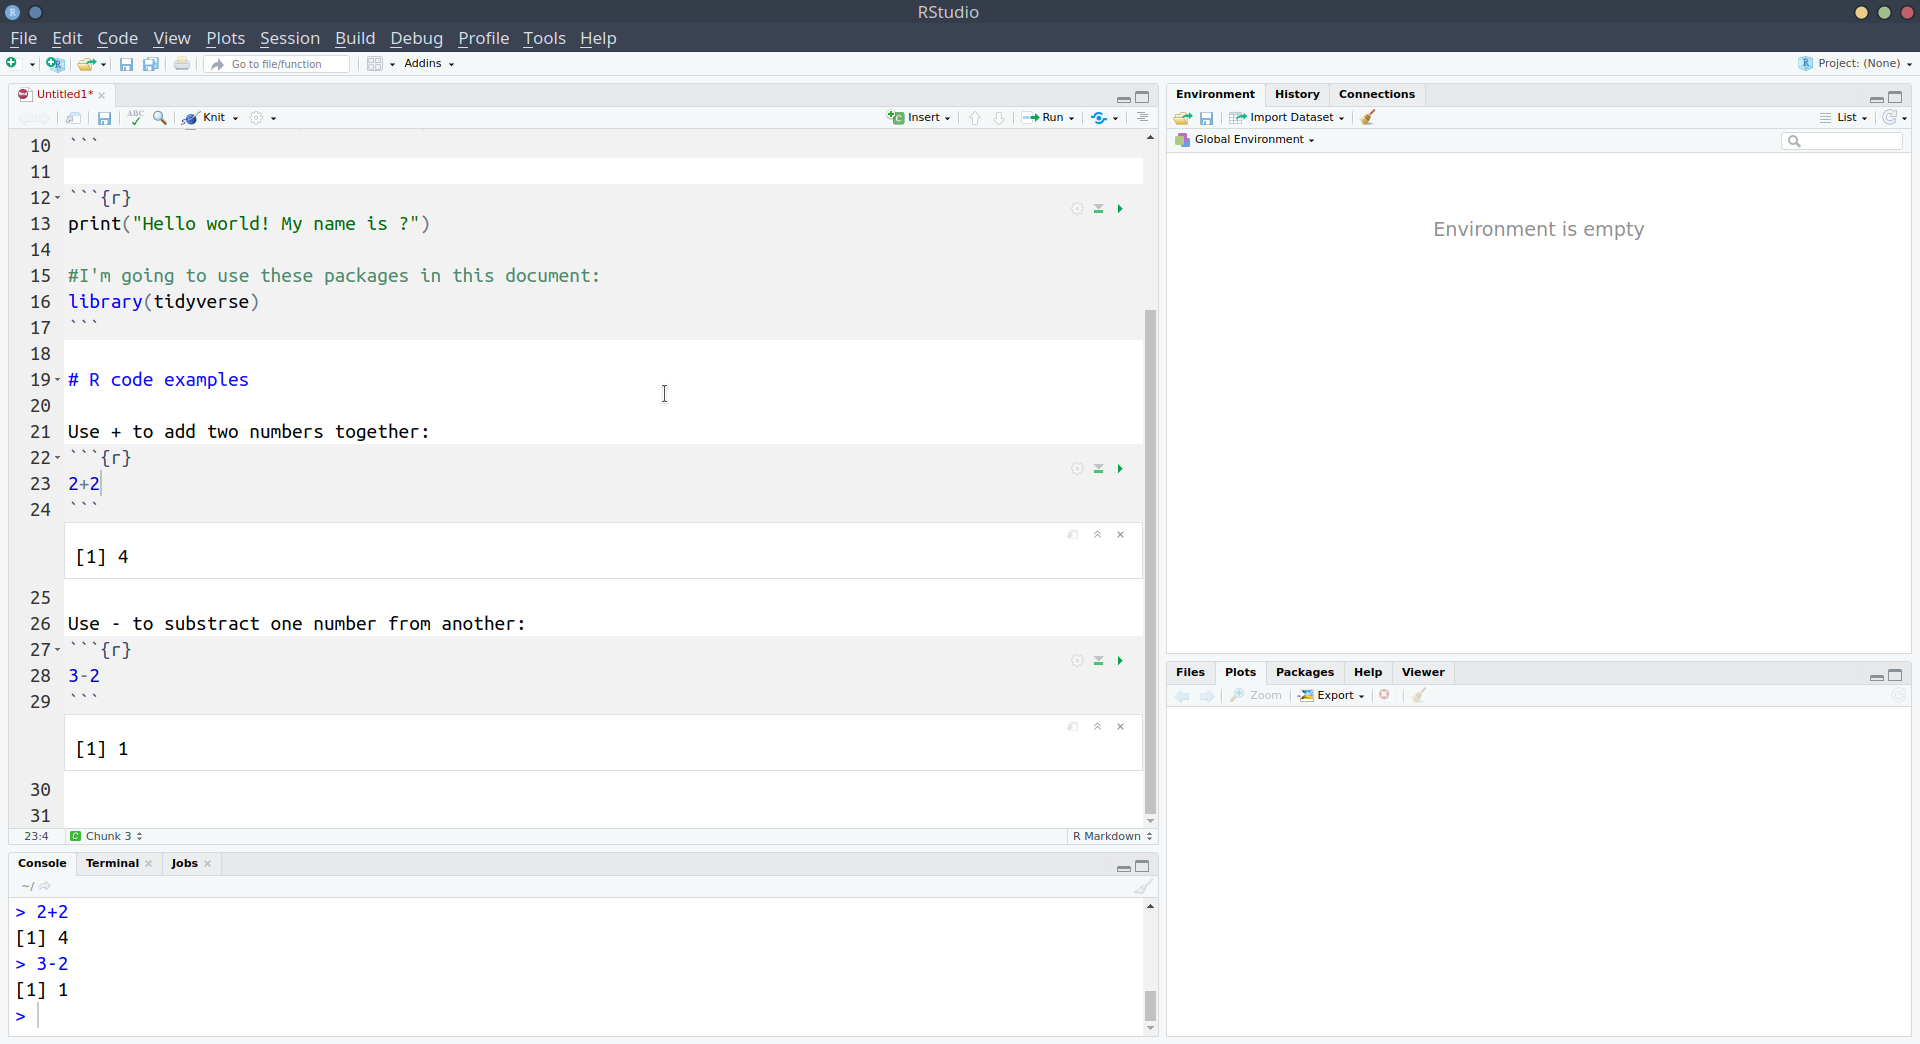
\includegraphics{images/installing_intro/ss_examples.png}

\hypertarget{storing-data-in-r-sequences-vectors-of-values}{%
\subsection*{Storing data in R: Sequences (``Vectors'') of values}\label{storing-data-in-r-sequences-vectors-of-values}}
\addcontentsline{toc}{subsection}{Storing data in R: Sequences (``Vectors'') of values}

We've already seen how to assign a value to a name/symbol using \texttt{\textless{}-}.\\
However, we've only seen how to assign a single number, e.g, \texttt{x\textless{}-5}.

To assign a sequence of values to R, we combine the values using \texttt{c()}.

\begin{Shaded}
\begin{Highlighting}[]
\NormalTok{myfirstvector <-}\StringTok{ }\KeywordTok{c}\NormalTok{(}\DecValTok{1}\NormalTok{,}\DecValTok{5}\NormalTok{,}\DecValTok{3}\NormalTok{,}\DecValTok{7}\NormalTok{)}
\NormalTok{myfirstvector}
\end{Highlighting}
\end{Shaded}

\begin{verbatim}
[1] 1 5 3 7
\end{verbatim}

We can perform arithmetic operations to each value in the vector:

\begin{Shaded}
\begin{Highlighting}[]
\NormalTok{myfirstvector }\OperatorTok{+}\StringTok{ }\DecValTok{5}
\end{Highlighting}
\end{Shaded}

\begin{verbatim}
[1]  6 10  8 12
\end{verbatim}

Values don't have to be numbers, but note what happens when we try to add 5 to a sequence which includes some non-numbers:

\begin{Shaded}
\begin{Highlighting}[]
\NormalTok{mysecondvector <-}\StringTok{ }\KeywordTok{c}\NormalTok{(}\DecValTok{1}\NormalTok{,}\DecValTok{4}\NormalTok{,}\StringTok{"cat"}\NormalTok{,}\StringTok{"dog"}\NormalTok{,}\StringTok{"parrot"}\NormalTok{,}\StringTok{"peppapig"}\NormalTok{)}
\NormalTok{mysecondvector }\OperatorTok{+}\StringTok{ }\DecValTok{5}
\end{Highlighting}
\end{Shaded}

Error in mysecondvector + 5 : non-numeric argument to binary operator

\hypertarget{reading-in-data}{%
\subsection*{Reading in data}\label{reading-in-data}}
\addcontentsline{toc}{subsection}{Reading in data}

While we can manually input data like we did above, more often, we will need to read in data which has been created elsewhere (like in excel, or by some software which is used to present participants with experiments).

\textbf{Task}
Add a new heading by typing the following:

\# Reading and storing data

\textbf{Remember:} We make headings using the \# \emph{outside} of a code chunk.

\textbf{Task}
Open Microsoft Excel, or LibreOffice Calc, or whatever spreadsheet software you have available to you, and create some data with more than one variable.

It can be whatever you want, but we've used a very small example here for you to follow, so feel free to use it if you like.

We've got two sets of values here: the names and the birth-years of each member of the beatles. The easiest way to think of this would be to have a row for each Beatle, and a column for each of name and birth-year.

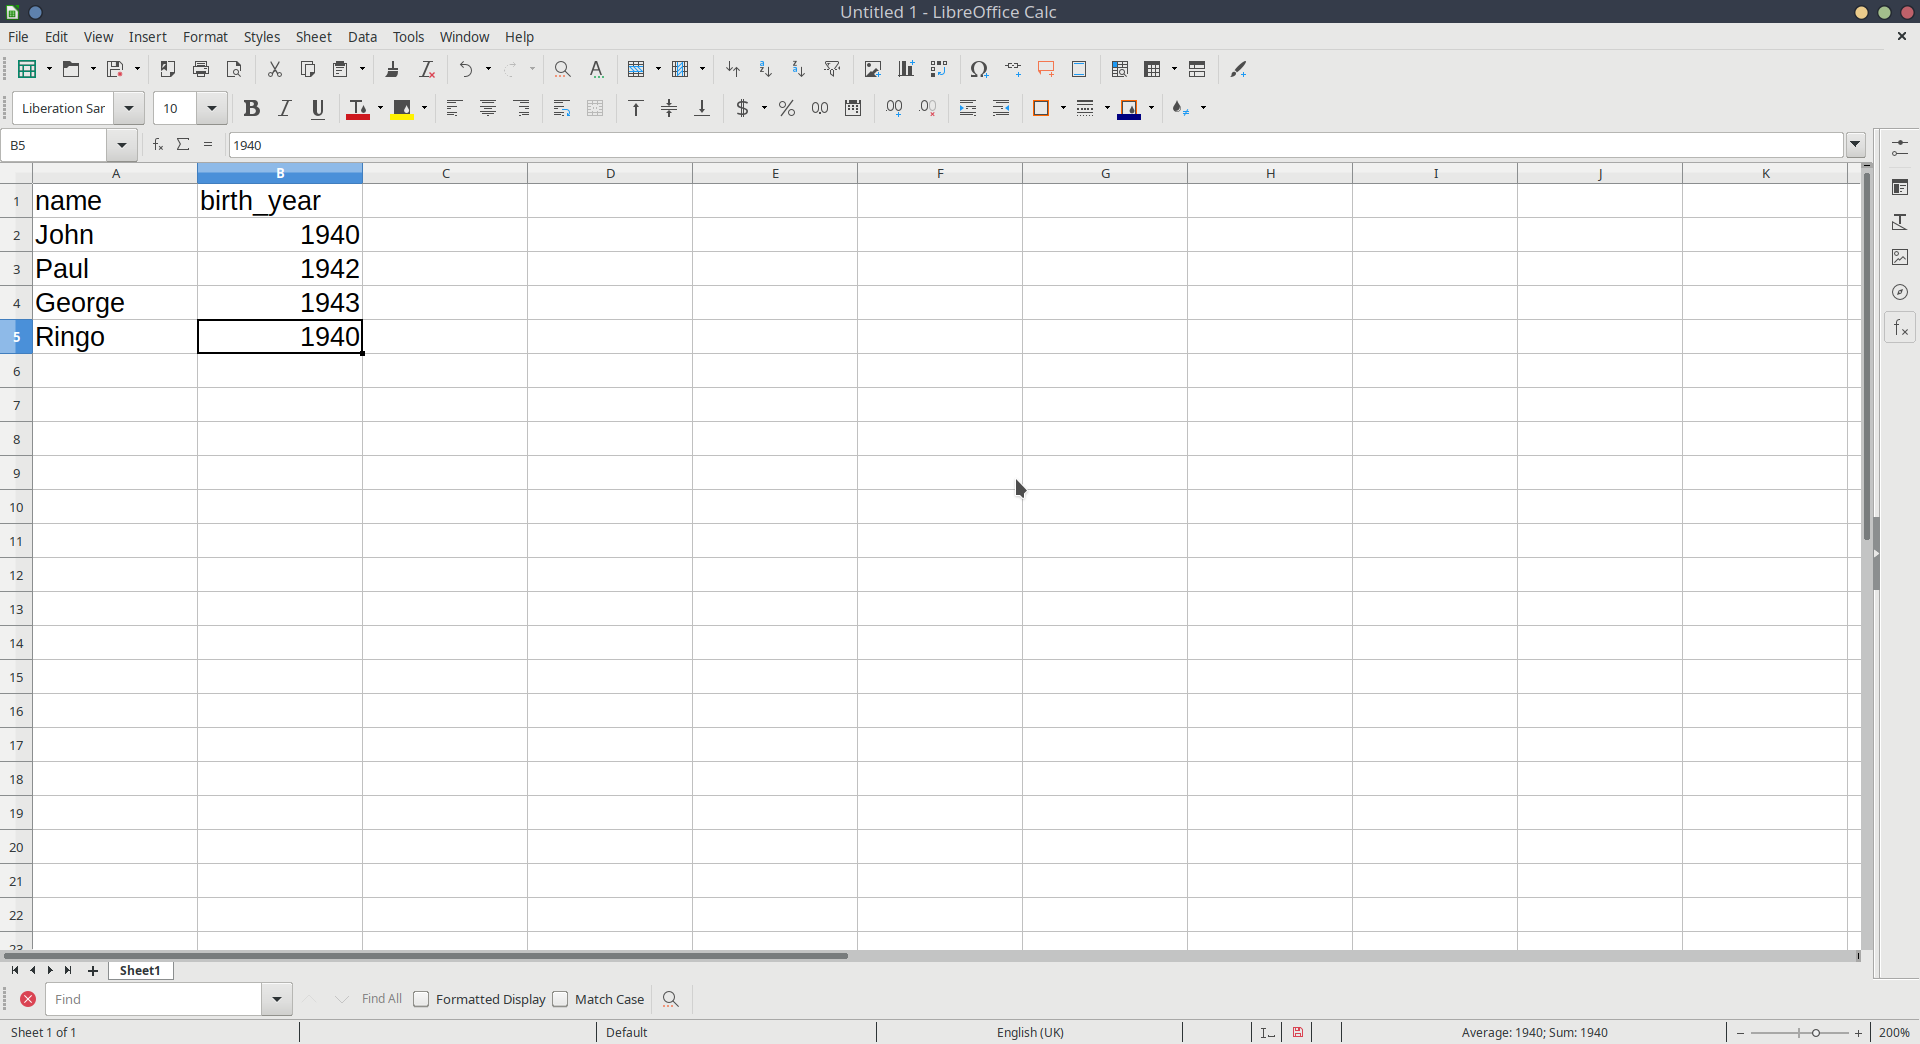
\includegraphics{images/installing_intro/create_data.png}

\textbf{Task}
Save the data as a \textbf{.csv} file.

Although R can read data when it's saved in Microsoft/LibreOffice formats, the simplest, and most universal way to save data is as simple text, with the values separated by some character - \textbf{.csv} stands for \textbf{comma separated values}.

In Microsoft Excel, if you go to:
\textbf{File \textgreater{} Save as}\\
In the Save as Type box, choose to save the file as \textbf{CSV (Comma delimited)}.

\textbf{Important:} save your data in the project folder you created at the start of this lab.

Back in Rstudio\ldots{}

Next, we're going to read the data into R. We can do this by using the \texttt{read\_csv()} function, and directing it to the file you just saved.

\textbf{Task}
Create a new code-chunk in your Rmarkdown, and in the chunk, type:
\texttt{read\_csv("name-of-your-data.csv")}, where you replace \emph{name-of-your-data} with whatever you just saved your data as in your spreadsheet software.

\textbf{Helpful tip}

If you have your text-cursor inside the quotation marks, and press the tab key on your keyboard, it will show you the files inside your project. You can then use the arrow keys to choose between them and press enter to add the code:

TODO - screencap gif

When you run the line of code you just wrote, it will print out the data, but will not store it. To do that, we need to assign it as something:

\begin{Shaded}
\begin{Highlighting}[]
\NormalTok{beatles <-}\StringTok{ }\KeywordTok{read_csv}\NormalTok{(}\StringTok{"data_from_excel.csv"}\NormalTok{)}
\end{Highlighting}
\end{Shaded}

Note that this will now turn up in the \emph{Environment} pane of Rstudio.

Now that we've got our data in R, we can print it out by simply using its name:

\begin{Shaded}
\begin{Highlighting}[]
\NormalTok{beatles}
\end{Highlighting}
\end{Shaded}

\begin{verbatim}
# A tibble: 4 x 2
  name   birth_year
  <chr>       <dbl>
1 John         1940
2 Paul         1942
3 George       1943
4 Ringo        1940
\end{verbatim}

And we can do things such as ask R how many rows and columns there are:

\begin{Shaded}
\begin{Highlighting}[]
\KeywordTok{dim}\NormalTok{(beatles)}
\end{Highlighting}
\end{Shaded}

\begin{verbatim}
[1] 4 2
\end{verbatim}

\begin{Shaded}
\begin{Highlighting}[]
\KeywordTok{str}\NormalTok{(beatles)}
\end{Highlighting}
\end{Shaded}

\begin{verbatim}
Classes 'spec_tbl_df', 'tbl_df', 'tbl' and 'data.frame':    4 obs. of  2 variables:
 $ name      : chr  "John" "Paul" "George" "Ringo"
 $ birth_year: num  1940 1942 1943 1940
 - attr(*, "spec")=
  .. cols(
  ..   name = col_character(),
  ..   birth_year = col_double()
  .. )
\end{verbatim}

\textbf{Task}
Use \texttt{dim()} to confirm how many rows and columns are in your data.

Use \texttt{str()} to take a look at the structure of the data.\\
Don't worry about the output of \texttt{str()} right now, we'll pick up with this in the next chapter.

\begin{center}\rule{0.5\linewidth}{0.5pt}\end{center}

\textbf{Task}
By now, you should have an Rmardkown document ( \textbf{.Rmd} ) with your answers to the tasks we've been through today.

Compile the document by clicking on the \textbf{Knit} button at the top (it will ask you to save your document first). The little arrow to the right of the Knit button allows you to compile to either \textbf{.pdf} or \textbf{.html}.

\textbf{Checklist for today}

\begin{enumerate}
\def\labelenumi{\arabic{enumi}.}
\tightlist
\item
  \textbf{EITHER:}

  \begin{itemize}
  \tightlist
  \item
    Option A: Install R and Rstudio   ✔
  \item
    Option B: Register for RstudioCloud (free) and log in   ✔
  \end{itemize}
\item
  Start a new project for the course   ✔
\item
  Change a few Rstudio settings (recommended)   ✔
\item
  Install some R packages (the ``tidyverse'')   ✔
\item
  Create a new Rmarkdown document   ✔
\item
  Complete today's tasks and exercises   ✔
\item
  Compile your Rmarkdown document   ✔
\item
  Celebrate!   ✔ 🎉
\end{enumerate}

\hypertarget{glossary}{%
\section*{Glossary}\label{glossary}}
\addcontentsline{toc}{section}{Glossary}

\begin{itemize}
\tightlist
\item
  console
\item
  environment
\item
  editor
\item
  r script
\item
  rmarkdown
\end{itemize}

\begin{longtable}[]{@{}rrr@{}}
\toprule
\begin{minipage}[b]{0.30\columnwidth}\raggedleft
Symbol\strut
\end{minipage} & \begin{minipage}[b]{0.30\columnwidth}\raggedleft
Description\strut
\end{minipage} & \begin{minipage}[b]{0.30\columnwidth}\raggedleft
Example\strut
\end{minipage}\tabularnewline
\midrule
\endhead
\begin{minipage}[t]{0.30\columnwidth}\raggedleft
\texttt{+}\strut
\end{minipage} & \begin{minipage}[t]{0.30\columnwidth}\raggedleft
Adds two numbers together\strut
\end{minipage} & \begin{minipage}[t]{0.30\columnwidth}\raggedleft
\texttt{2+2} - two plus two\strut
\end{minipage}\tabularnewline
\begin{minipage}[t]{0.30\columnwidth}\raggedleft
\texttt{-}\strut
\end{minipage} & \begin{minipage}[t]{0.30\columnwidth}\raggedleft
Subtract one number from another\strut
\end{minipage} & \begin{minipage}[t]{0.30\columnwidth}\raggedleft
\texttt{3-1} - three minus one\strut
\end{minipage}\tabularnewline
\begin{minipage}[t]{0.30\columnwidth}\raggedleft
\texttt{*}\strut
\end{minipage} & \begin{minipage}[t]{0.30\columnwidth}\raggedleft
Multiply two numbers together\strut
\end{minipage} & \begin{minipage}[t]{0.30\columnwidth}\raggedleft
\texttt{3*3} - three times three\strut
\end{minipage}\tabularnewline
\begin{minipage}[t]{0.30\columnwidth}\raggedleft
\texttt{/}\strut
\end{minipage} & \begin{minipage}[t]{0.30\columnwidth}\raggedleft
Divide one number by another\strut
\end{minipage} & \begin{minipage}[t]{0.30\columnwidth}\raggedleft
\texttt{9/3} - nine divided by three\strut
\end{minipage}\tabularnewline
\begin{minipage}[t]{0.30\columnwidth}\raggedleft
\texttt{()}\strut
\end{minipage} & \begin{minipage}[t]{0.30\columnwidth}\raggedleft
group operations together\strut
\end{minipage} & \begin{minipage}[t]{0.30\columnwidth}\raggedleft
\texttt{(2+2)/4} is different from \texttt{2+2/4}\strut
\end{minipage}\tabularnewline
\begin{minipage}[t]{0.30\columnwidth}\raggedleft
\texttt{\^{}}\strut
\end{minipage} & \begin{minipage}[t]{0.30\columnwidth}\raggedleft
to the power of..\strut
\end{minipage} & \begin{minipage}[t]{0.30\columnwidth}\raggedleft
\texttt{4\^{}2} - four to the power of two, or four squared\strut
\end{minipage}\tabularnewline
\begin{minipage}[t]{0.30\columnwidth}\raggedleft
\texttt{\textless{}-}\strut
\end{minipage} & \begin{minipage}[t]{0.30\columnwidth}\raggedleft
stores an object in R with the left hand side (LHS) as the name, and the RHS as the value\strut
\end{minipage} & \begin{minipage}[t]{0.30\columnwidth}\raggedleft
\texttt{x\textless{}-10}\strut
\end{minipage}\tabularnewline
\begin{minipage}[t]{0.30\columnwidth}\raggedleft
\texttt{=}\strut
\end{minipage} & \begin{minipage}[t]{0.30\columnwidth}\raggedleft
stores an object in R with the left hand side (LHS) as the name, and the RHS as the value\strut
\end{minipage} & \begin{minipage}[t]{0.30\columnwidth}\raggedleft
\texttt{x\ =\ 10}\strut
\end{minipage}\tabularnewline
\begin{minipage}[t]{0.30\columnwidth}\raggedleft
\texttt{\textless{}}\strut
\end{minipage} & \begin{minipage}[t]{0.30\columnwidth}\raggedleft
is less than?\strut
\end{minipage} & \begin{minipage}[t]{0.30\columnwidth}\raggedleft
\texttt{2\textless{}3}\strut
\end{minipage}\tabularnewline
\begin{minipage}[t]{0.30\columnwidth}\raggedleft
\texttt{\textgreater{}}\strut
\end{minipage} & \begin{minipage}[t]{0.30\columnwidth}\raggedleft
is greater than?\strut
\end{minipage} & \begin{minipage}[t]{0.30\columnwidth}\raggedleft
\texttt{2\textgreater{}3}\strut
\end{minipage}\tabularnewline
\begin{minipage}[t]{0.30\columnwidth}\raggedleft
\texttt{\textless{}=}\strut
\end{minipage} & \begin{minipage}[t]{0.30\columnwidth}\raggedleft
is less than or equal to?\strut
\end{minipage} & \begin{minipage}[t]{0.30\columnwidth}\raggedleft
\texttt{2\textless{}=3}\strut
\end{minipage}\tabularnewline
\begin{minipage}[t]{0.30\columnwidth}\raggedleft
\texttt{\textgreater{}=}\strut
\end{minipage} & \begin{minipage}[t]{0.30\columnwidth}\raggedleft
is greater than or equal to?\strut
\end{minipage} & \begin{minipage}[t]{0.30\columnwidth}\raggedleft
\texttt{2\textgreater{}=2}\strut
\end{minipage}\tabularnewline
\begin{minipage}[t]{0.30\columnwidth}\raggedleft
\texttt{==}\strut
\end{minipage} & \begin{minipage}[t]{0.30\columnwidth}\raggedleft
is equal to?\strut
\end{minipage} & \begin{minipage}[t]{0.30\columnwidth}\raggedleft
\texttt{(5+5)\ ==\ 10}\strut
\end{minipage}\tabularnewline
\begin{minipage}[t]{0.30\columnwidth}\raggedleft
\texttt{!=}\strut
\end{minipage} & \begin{minipage}[t]{0.30\columnwidth}\raggedleft
is not equal to?\strut
\end{minipage} & \begin{minipage}[t]{0.30\columnwidth}\raggedleft
\texttt{(2+3)\ !=\ 4}\strut
\end{minipage}\tabularnewline
\begin{minipage}[t]{0.30\columnwidth}\raggedleft
\texttt{c()}\strut
\end{minipage} & \begin{minipage}[t]{0.30\columnwidth}\raggedleft
combines values into a vector (a sequence of values)\strut
\end{minipage} & \begin{minipage}[t]{0.30\columnwidth}\raggedleft
\texttt{c(1,2,3,4)}\strut
\end{minipage}\tabularnewline
\bottomrule
\end{longtable}

\hypertarget{chap-data-types}{%
\chapter{Types of data}\label{chap-data-types}}

\hypertarget{learning-objectives-1}{%
\section*{Learning Objectives}\label{learning-objectives-1}}
\addcontentsline{toc}{section}{Learning Objectives}

\begin{itemize}
\tightlist
\item
  LO1: Learn how to access variables in a dataframe in R\\
\item
  LO2: Understand the distinction between types of variables\\
\item
  LO3: Learn how to code data as different types (classes) in R
\end{itemize}

So we've got R and Rstudio installed, and we know how to read in data from an external source, and do some basic arithmetic operations.

We're going to now take a look at how to pull out specific pieces of data, before we move on to talking about different types of data.

\hypertarget{accessing-subsections-of-data}{%
\section{Accessing subsections of data}\label{accessing-subsections-of-data}}

Suppose we read some data in to R:

\begin{Shaded}
\begin{Highlighting}[]
\NormalTok{some_data<-dplyr}\OperatorTok{::}\NormalTok{starwars }\OperatorTok\StringTok{ }\KeywordTok{select}\NormalTok{(}\OperatorTok{-}\NormalTok{mass, }\OperatorTok{-}\NormalTok{skin_color, }\OperatorTok{-}\NormalTok{films, }\OperatorTok{-}\NormalTok{vehicles,}\OperatorTok{-}\NormalTok{starships, }\OperatorTok{-}\NormalTok{gender,}\OperatorTok{-}\NormalTok{birth_year)}
\NormalTok{some_data[}\DecValTok{87}\NormalTok{,]<-}\KeywordTok{c}\NormalTok{(}\StringTok{"Homer Simpson"}\NormalTok{,}\DecValTok{180}\NormalTok{,}\OtherTok{NA}\NormalTok{,}\OtherTok{NA}\NormalTok{,}\StringTok{"Springfield"}\NormalTok{,}\StringTok{"unknown"}\NormalTok{)}
\NormalTok{some_data[}\DecValTok{2}\NormalTok{,}\StringTok{"species"}\NormalTok{]<-}\StringTok{"Human"}
\NormalTok{some_data[}\DecValTok{7}\NormalTok{,}\StringTok{"height"}\NormalTok{]<-}\DecValTok{9420}
\end{Highlighting}
\end{Shaded}

\textbf{Reading data from the internet}

Note that when you have a url for some data, such as \href{url}{link}, you can read it in directly by giving functions like \texttt{read\_csv()} the url inside quotation marks.

We can print out the top of the data by using the name we just gave it:

\begin{Shaded}
\begin{Highlighting}[]
\NormalTok{some_data}
\end{Highlighting}
\end{Shaded}

\begin{verbatim}
# A tibble: 87 x 6
   name               height hair_color    eye_color homeworld species
   <chr>              <chr>  <chr>         <chr>     <chr>     <chr>  
 1 Luke Skywalker     172    blond         blue      Tatooine  Human  
 2 C-3PO              167    <NA>          yellow    Tatooine  Human  
 3 R2-D2              96     <NA>          red       Naboo     Droid  
 4 Darth Vader        202    none          yellow    Tatooine  Human  
 5 Leia Organa        150    brown         brown     Alderaan  Human  
 6 Owen Lars          178    brown, grey   blue      Tatooine  Human  
 7 Beru Whitesun lars 9420   brown         blue      Tatooine  Human  
 8 R5-D4              97     <NA>          red       Tatooine  Droid  
 9 Biggs Darklighter  183    black         brown     Tatooine  Human  
10 Obi-Wan Kenobi     182    auburn, white blue-gray Stewjon   Human  
# ... with 77 more rows
\end{verbatim}

The data contains information on various characteristics of characters from Star Wars.

\textbf{Tip:} Try clicking on the data in your \textbf{environment} (the top right window of Rstudio). It will open the data in a tab in the editor window - this is another way of looking at the data, more like you would in spreadsheet software like Microsoft Excel.

We can take a look at how big the data is (the dimensions), using \texttt{dim()}

\begin{Shaded}
\begin{Highlighting}[]
\KeywordTok{dim}\NormalTok{(some_data)}
\end{Highlighting}
\end{Shaded}

\begin{verbatim}
[1] 87  6
\end{verbatim}

There's a reasonable amount of data in there - 87 rows and 6 variables (columns). What if we want to extract certain bits of it?

This is where we learn about two important bits of R code used to access parts of data - the dollar sign \texttt{\$}, and the square brackets \texttt{{[}{]}}.

\hypertarget{the-dollar-sign}{%
\subsubsection*{The dollar sign \$}\label{the-dollar-sign}}
\addcontentsline{toc}{subsubsection}{The dollar sign \$}

The dollar sign allows us to select a specific variable.\\
For instance, we can pull out the variable named ``eye\_color'' in the data, by using \texttt{\$eye\_color} after the name that we gave our dataset:

\begin{Shaded}
\begin{Highlighting}[]
\NormalTok{some_data}\OperatorTok{$}\NormalTok{eye_color}
\end{Highlighting}
\end{Shaded}

\begin{verbatim}
 [1] "blue"          "yellow"        "red"           "yellow"        "brown"         "blue"          "blue"         
 [8] "red"           "brown"         "blue-gray"     "blue"          "blue"          "blue"          "brown"        
[15] "black"         "orange"        "hazel"         "blue"          "brown"         "yellow"        "brown"        
[22] "red"           "red"           "brown"         "blue"          "orange"        "blue"          "brown"        
[29] "brown"         "black"         "blue"          "red"           "blue"          "orange"        "orange"       
[36] "orange"        "blue"          "yellow"        "orange"        "brown"         "brown"         "yellow"       
[43] "pink"          "hazel"         "yellow"        "black"         "orange"        "brown"         "yellow"       
[50] "black"         "brown"         "blue"          "orange"        "yellow"        "black"         "blue"         
[57] "brown"         "brown"         "blue"          "yellow"        "blue"          "blue"          "brown"        
[64] "brown"         "brown"         "brown"         "yellow"        "yellow"        "black"         "black"        
[71] "blue"          "unknown"       "red, blue"     "unknown"       "gold"          "black"         "green, yellow"
[78] "blue"          "brown"         "white"         "black"         "dark"          "hazel"         "brown"        
[85] "black"         "unknown"       NA             
\end{verbatim}

\hypertarget{the-square-brackets}{%
\subsubsection*{The square brackets {[}{]}}\label{the-square-brackets}}
\addcontentsline{toc}{subsubsection}{The square brackets {[}{]}}

Square brackets are used to do what is known as \textbf{indexing} (finding specific entries in your data).

We can retrieve bits of data by identifying the \(i^{th}\) entry(s) inside the square brackets, for instance:

\begin{Shaded}
\begin{Highlighting}[]
\NormalTok{somevalues <-}\StringTok{ }\KeywordTok{c}\NormalTok{(}\DecValTok{10}\NormalTok{,}\DecValTok{20}\NormalTok{,}\DecValTok{30}\NormalTok{,}\DecValTok{40}\NormalTok{,}\DecValTok{50}\NormalTok{,}\DecValTok{60}\NormalTok{,}\DecValTok{70}\NormalTok{,}\DecValTok{80}\NormalTok{,}\DecValTok{90}\NormalTok{,}\DecValTok{100}\NormalTok{)}

\CommentTok{# pull out the 3rd entry}
\NormalTok{somevalues[}\DecValTok{3}\NormalTok{]}
\end{Highlighting}
\end{Shaded}

\begin{verbatim}
[1] 30
\end{verbatim}

In the above example, we have a \textbf{vector} (a single sequence of values), and so we can retrieve entries with the syntax:\\
\emph{vector{[}entry{]}}

In a \textbf{dataframe} we have an extra dimension - we have \emph{rows} \textbf{and} \emph{columns}.
Using square brackets with a dataframe needs us to specify both:
\emph{dataframe{[}rows, columns{]}}

For instance:

\begin{Shaded}
\begin{Highlighting}[]
\CommentTok{# first row, fourth column:}
\NormalTok{some_data[}\DecValTok{1}\NormalTok{,}\DecValTok{4}\NormalTok{]}
\end{Highlighting}
\end{Shaded}

\begin{verbatim}
# A tibble: 1 x 1
  eye_color
  <chr>    
1 blue     
\end{verbatim}

\begin{Shaded}
\begin{Highlighting}[]
\CommentTok{# tenth row, first column:}
\NormalTok{some_data[}\DecValTok{10}\NormalTok{,}\DecValTok{1}\NormalTok{]}
\end{Highlighting}
\end{Shaded}

\begin{verbatim}
# A tibble: 1 x 1
  name          
  <chr>         
1 Obi-Wan Kenobi
\end{verbatim}

If we leave either rows or columns blank, then we will get out \emph{all} of them:

\begin{Shaded}
\begin{Highlighting}[]
\CommentTok{# tenth row, all columns:}
\NormalTok{some_data[}\DecValTok{10}\NormalTok{, ]}
\end{Highlighting}
\end{Shaded}

\begin{verbatim}
# A tibble: 1 x 6
  name           height hair_color    eye_color homeworld species
  <chr>          <chr>  <chr>         <chr>     <chr>     <chr>  
1 Obi-Wan Kenobi 182    auburn, white blue-gray Stewjon   Human  
\end{verbatim}

\begin{Shaded}
\begin{Highlighting}[]
\CommentTok{# all rows, 2nd column:}
\NormalTok{some_data[ , }\DecValTok{2}\NormalTok{]}
\end{Highlighting}
\end{Shaded}

\begin{verbatim}
# A tibble: 87 x 1
   height
   <chr> 
 1 172   
 2 167   
 3 96    
 4 202   
 5 150   
 6 178   
 7 9420  
 8 97    
 9 183   
10 182   
# ... with 77 more rows
\end{verbatim}

There are is another way to identify column - we can use the name in quotation marks:

\begin{Shaded}
\begin{Highlighting}[]
\CommentTok{# first row, "species" column}
\NormalTok{some_data[}\DecValTok{1}\NormalTok{, }\StringTok{"species"}\NormalTok{]}
\end{Highlighting}
\end{Shaded}

\begin{verbatim}
# A tibble: 1 x 1
  species
  <chr>  
1 Human  
\end{verbatim}

Finally, we can also ask for multiple rows, or multiple columns, or both!

\begin{Shaded}
\begin{Highlighting}[]
\CommentTok{# the 1st AND the 6th row, }
\CommentTok{# and the 1st AND 3rd columns:}
\NormalTok{some_data[}\KeywordTok{c}\NormalTok{(}\DecValTok{1}\NormalTok{,}\DecValTok{6}\NormalTok{), }\KeywordTok{c}\NormalTok{(}\DecValTok{1}\NormalTok{,}\DecValTok{3}\NormalTok{)]}
\end{Highlighting}
\end{Shaded}

\begin{verbatim}
# A tibble: 2 x 2
  name           hair_color 
  <chr>          <chr>      
1 Luke Skywalker blond      
2 Owen Lars      brown, grey
\end{verbatim}

And we can specify a sequence using the colon, \texttt{from:to}:

\begin{Shaded}
\begin{Highlighting}[]
\CommentTok{# FROM the 1st TO the 6th row, all columns:}
\NormalTok{some_data[}\DecValTok{1}\OperatorTok{:}\DecValTok{6}\NormalTok{, ]}
\end{Highlighting}
\end{Shaded}

\begin{verbatim}
# A tibble: 6 x 6
  name           height hair_color  eye_color homeworld species
  <chr>          <chr>  <chr>       <chr>     <chr>     <chr>  
1 Luke Skywalker 172    blond       blue      Tatooine  Human  
2 C-3PO          167    <NA>        yellow    Tatooine  Human  
3 R2-D2          96     <NA>        red       Naboo     Droid  
4 Darth Vader    202    none        yellow    Tatooine  Human  
5 Leia Organa    150    brown       brown     Alderaan  Human  
6 Owen Lars      178    brown, grey blue      Tatooine  Human  
\end{verbatim}

\textbf{Extra}
We can use the two accessors in combination:

\begin{Shaded}
\begin{Highlighting}[]
\CommentTok{# extract the variable called "name" and show the 20th entry }
\NormalTok{some_data}\OperatorTok{$}\NormalTok{name[}\DecValTok{20}\NormalTok{]}
\end{Highlighting}
\end{Shaded}

\begin{verbatim}
[1] "Palpatine"
\end{verbatim}

\textbf{Note:} When we do this, we don't have the comma inside the square brackets.\\
When we use the \texttt{\$} to pull out a variable, such as \texttt{some\_data\$name}, we no longer have a dataframe - \texttt{some\_data\$name} doesn't have rows and columns, it just has a series of values - \emph{it's a vector!}.\\
So when you are using \texttt{{[}{]}} with a \textbf{vector} (1 dimension) rather than a \textbf{dataframe} (2 dimensions), you don't specify \texttt{{[}rows,\ columns{]}}, but simply \texttt{{[}entry{]}}.

\hypertarget{accessors}{%
\subsubsection*{Accessors}\label{accessors}}
\addcontentsline{toc}{subsubsection}{Accessors}

\textbf{The dollar sign \$}

Used to extract a variable from a dataframe:

\begin{itemize}
\tightlist
\item
  \texttt{dataframe\$variable}
\end{itemize}

\textbf{The square brackets {[}{]}}

Used to extract parts of an R object by identifying rows and/or columns, or more generally, ``entries''. Left blank will return all.

\begin{itemize}
\tightlist
\item
  \texttt{dataframe{[}rows,\ columns{]}}~\\
\item
  \texttt{vector{[}entries{]}}
\end{itemize}

\begin{center}\rule{0.5\linewidth}{0.5pt}\end{center}

\hypertarget{editing-subsections-of-data}{%
\section{Editing subsections of data}\label{editing-subsections-of-data}}

Now that we've seen how to \emph{access} sections of data, we can learn how to edit them!

\textbf{Data Cleaning}

One of the most common reasons you will need to edit entries in your data is in \textbf{data cleaning}. This is the process of identifying incorrect/incomplete/irrelevant data, and replacing/modifying/deleting them.

\hypertarget{modifying-specific-entries}{%
\subsection*{Modifying specific entries}\label{modifying-specific-entries}}
\addcontentsline{toc}{subsection}{Modifying specific entries}

single entries
{[}{]}\textless{}-

\hypertarget{changing-a-whole-column}{%
\subsection*{Changing a whole column}\label{changing-a-whole-column}}
\addcontentsline{toc}{subsection}{Changing a whole column}

change heights from centimeters to meters
\$ \textless{}

\hypertarget{removing-rowscolumns}{%
\subsection*{Removing rows/columns}\label{removing-rowscolumns}}
\addcontentsline{toc}{subsection}{Removing rows/columns}

editing the whole data - e.g., removing a row

think of it as ``overwriting''

\hypertarget{types-of-data}{%
\section{Types of data}\label{types-of-data}}

table - descriptions from lectures

\begin{longtable}[]{@{}rrr@{}}
\toprule
\begin{minipage}[b]{0.30\columnwidth}\raggedleft
\textbf{Type}\strut
\end{minipage} & \begin{minipage}[b]{0.30\columnwidth}\raggedleft
\textbf{Description}\strut
\end{minipage} & \begin{minipage}[b]{0.30\columnwidth}\raggedleft
\textbf{Example}\strut
\end{minipage}\tabularnewline
\midrule
\endhead
\begin{minipage}[t]{0.30\columnwidth}\raggedleft
\textbf{Categorical}\strut
\end{minipage} & \begin{minipage}[t]{0.30\columnwidth}\raggedleft
Variables with a discrete number of response optionsBinary data is a special case with only 2 possible values\strut
\end{minipage} & \begin{minipage}[t]{0.30\columnwidth}\raggedleft
Species: \emph{Human}, \emph{Droid}, \emph{Wookie}, \emph{Hutt}, \ldots{}Is\_Human: \emph{Yes}, \emph{No}.\strut
\end{minipage}\tabularnewline
\begin{minipage}[t]{0.30\columnwidth}\raggedleft
\textbf{Continuous}\strut
\end{minipage} & \begin{minipage}[t]{0.30\columnwidth}\raggedleft
Variables which can take any real number value within the specified range of measurement\strut
\end{minipage} & \begin{minipage}[t]{0.30\columnwidth}\raggedleft
Height: \emph{172}, \emph{165.2}, \emph{183}, \ldots{}\strut
\end{minipage}\tabularnewline
\begin{minipage}[t]{0.30\columnwidth}\raggedleft
\textbf{Count}\strut
\end{minipage} & \begin{minipage}[t]{0.30\columnwidth}\raggedleft
Variables which can only take non-negative integer values (0,1,2,3 etc.)\strut
\end{minipage} & \begin{minipage}[t]{0.30\columnwidth}\raggedleft
Number\_of\_limbs\_lost: \emph{1}, \emph{0}, \emph{0}, \emph{1}, \emph{4}, \ldots{}\strut
\end{minipage}\tabularnewline
\bottomrule
\end{longtable}

In R, different types of data get treated differently by functions, and often we need to tell R explicitly what type of data each variable is.

\begin{longtable}[]{@{}rrr@{}}
\toprule
\textbf{Type} & \textbf{Set as\ldots{}} & \textbf{Check is\ldots{}}\tabularnewline
\midrule
\endhead
\textbf{Categorical} & \texttt{as.factor()}\texttt{factor()} & \texttt{is.factor(variable)}\tabularnewline
\textbf{Continuous} & \texttt{as.numeric()} & \texttt{is.numeric(variable)}\tabularnewline
\textbf{Character} & \texttt{as.character()} & \texttt{is.character(variable)}\tabularnewline
\bottomrule
\end{longtable}

\begin{Shaded}
\begin{Highlighting}[]
\KeywordTok{distinct}\NormalTok{(some_data, species)}
\end{Highlighting}
\end{Shaded}

\begin{verbatim}
# A tibble: 39 x 1
   species       
   <chr>         
 1 Human         
 2 Droid         
 3 Wookiee       
 4 Rodian        
 5 Hutt          
 6 Yoda's species
 7 Trandoshan    
 8 Mon Calamari  
 9 Ewok          
10 Sullustan     
# ... with 29 more rows
\end{verbatim}

\begin{Shaded}
\begin{Highlighting}[]
\NormalTok{some_data <-}\StringTok{ }\KeywordTok{read_csv}\NormalTok{(}\StringTok{"https://raw.githubusercontent.com/rfordatascience/tidytuesday/master/data/2020/2020-01-14/passwords.csv"}\NormalTok{) }\OperatorTok\StringTok{ }\KeywordTok{select}\NormalTok{(rank, password, category, value, strength) }\OperatorTok
\StringTok{    }\KeywordTok{rename}\NormalTok{(}\DataTypeTok{cracked =} \StringTok{"value"}\NormalTok{)}

\KeywordTok{tibble}\NormalTok{(}
    \DataTypeTok{variable =} \KeywordTok{names}\NormalTok{(some_data),}
    \DataTypeTok{description =} \KeywordTok{c}\NormalTok{(}\StringTok{"popularity in their database of released passwords"}\NormalTok{,}
                    \StringTok{"password"}\NormalTok{,}\StringTok{"category"}\NormalTok{,}\StringTok{"Time to crack by online guessing"}\NormalTok{,}\StringTok{"Strength = quality of password where 10 is highest, 1 is lowest"}\NormalTok{)}
\NormalTok{) }\OperatorTok\StringTok{ }\NormalTok{knitr}\OperatorTok{::}\KeywordTok{kable}\NormalTok{()}
\end{Highlighting}
\end{Shaded}

\begin{tabular}{l|l}
\hline
variable & description\\
\hline
rank & popularity in their database of released passwords\\
\hline
password & password\\
\hline
category & category\\
\hline
cracked & Time to crack by online guessing\\
\hline
strength & Strength = quality of password where 10 is highest, 1 is lowest\\
\hline
\end{tabular}

\textbf{Task}
In a new code chunk, do the following:

\begin{enumerate}
\def\labelenumi{\arabic{enumi}.}
\tightlist
\item
  store the following numbers as an object in R:\\
  4,7,3,1,8,9,5,2,2,6,9,9,5,20\\
\item
  Try using the function \texttt{sum()}, with the name of your object inside the brackets.
\end{enumerate}

\textbf{Solution }
Because this is just a set of numbers, we store it as a \textbf{vector}, using \texttt{c()}.\\
We have named it \texttt{myvec}, but you can call yours whatever you like.

The \texttt{sum()} function will add all of the numbers together!

\begin{Shaded}
\begin{Highlighting}[]
\NormalTok{myvec <-}\StringTok{ }\KeywordTok{c}\NormalTok{(}\DecValTok{4}\NormalTok{,}\DecValTok{7}\NormalTok{,}\DecValTok{3}\NormalTok{,}\DecValTok{1}\NormalTok{,}\DecValTok{8}\NormalTok{,}\DecValTok{9}\NormalTok{,}\DecValTok{5}\NormalTok{,}\DecValTok{2}\NormalTok{,}\DecValTok{2}\NormalTok{,}\DecValTok{6}\NormalTok{,}\DecValTok{9}\NormalTok{,}\DecValTok{9}\NormalTok{,}\DecValTok{5}\NormalTok{,}\DecValTok{20}\NormalTok{)}
\KeywordTok{sum}\NormalTok{(myvec)}
\end{Highlighting}
\end{Shaded}

\begin{verbatim}
[1] 90
\end{verbatim}

\textbf{Task}
Using the square brackets - \texttt{{[}{]}} - pull out the 2nd, 4th and 6th values in the object you just created.

\textbf{Hint:} You will need to put inside the square brackets a \emph{sequence of} numbers. How do we combine numbers in to a sequence in R? using \texttt{c()}!

\textbf{Solution }

\begin{Shaded}
\begin{Highlighting}[]
\NormalTok{myvec[}\KeywordTok{c}\NormalTok{(}\DecValTok{2}\NormalTok{,}\DecValTok{4}\NormalTok{,}\DecValTok{6}\NormalTok{)]}
\end{Highlighting}
\end{Shaded}

\begin{verbatim}
[1] 7 1 9
\end{verbatim}

\textbf{Task}
Using the square brackets, show the 167th row, with all columns.

\textbf{Remember:} When you are using \texttt{{[}{]}} with a dataframe, you specify \texttt{data{[}rows,\ columns{]}}. If you leave either rows or columns blank it will give all of them - for instance, \texttt{data{[}\ ,\ columns{]}} will give you all rows for some specified columns.

\textbf{Solution }

\begin{Shaded}
\begin{Highlighting}[]
\NormalTok{mydata[}\DecValTok{167}\NormalTok{,]}
\end{Highlighting}
\end{Shaded}

\hypertarget{matrices}{%
\subsection*{Matrices}\label{matrices}}
\addcontentsline{toc}{subsection}{Matrices}

We will often have several vectors in which the 1st value of each vector corresponds to the same observation, for instance:

\begin{Shaded}
\begin{Highlighting}[]
\NormalTok{age<-}\KeywordTok{c}\NormalTok{(}\DecValTok{1}\NormalTok{,}\DecValTok{2}\NormalTok{,}\DecValTok{3}\NormalTok{,}\DecValTok{4}\NormalTok{,}\DecValTok{5}\NormalTok{)}
\NormalTok{height<-}\KeywordTok{c}\NormalTok{(}\DecValTok{20}\NormalTok{,}\DecValTok{70}\NormalTok{,}\DecValTok{80}\NormalTok{,}\DecValTok{90}\NormalTok{,}\DecValTok{95}\NormalTok{)}
\end{Highlighting}
\end{Shaded}

But these would be better stored as a ``Matrix''

\begin{Shaded}
\begin{Highlighting}[]
\KeywordTok{matrix}\NormalTok{(}\KeywordTok{c}\NormalTok{(}\DecValTok{1}\NormalTok{,}\DecValTok{2}\NormalTok{,}\DecValTok{3}\NormalTok{,}\DecValTok{4}\NormalTok{,}\DecValTok{5}\NormalTok{,}\DecValTok{20}\NormalTok{,}\DecValTok{70}\NormalTok{,}\DecValTok{80}\NormalTok{,}\DecValTok{90}\NormalTok{,}\DecValTok{95}\NormalTok{), }\DataTypeTok{nrow=}\DecValTok{5}\NormalTok{)}
\end{Highlighting}
\end{Shaded}

\begin{verbatim}
     [,1] [,2]
[1,]    1   20
[2,]    2   70
[3,]    3   80
[4,]    4   90
[5,]    5   95
\end{verbatim}

\hypertarget{glossary-1}{%
\section{Glossary}\label{glossary-1}}

\begin{itemize}
\tightlist
\item
  data cleaning
\end{itemize}

\begin{longtable}[]{@{}rrr@{}}
\toprule
\begin{minipage}[b]{0.30\columnwidth}\raggedleft
Symbol\strut
\end{minipage} & \begin{minipage}[b]{0.30\columnwidth}\raggedleft
Description\strut
\end{minipage} & \begin{minipage}[b]{0.30\columnwidth}\raggedleft
Example\strut
\end{minipage}\tabularnewline
\midrule
\endhead
\begin{minipage}[t]{0.30\columnwidth}\raggedleft
\texttt{{[}{]}}\strut
\end{minipage} & \begin{minipage}[t]{0.30\columnwidth}\raggedleft
used to extract the 1st, 2nd, \ldots{} \(i^{th}\) elements in a set of numbers\strut
\end{minipage} & \begin{minipage}[t]{0.30\columnwidth}\raggedleft
\texttt{myvector{[}3{]}}\strut
\end{minipage}\tabularnewline
\begin{minipage}[t]{0.30\columnwidth}\raggedleft
\texttt{\$}\strut
\end{minipage} & \begin{minipage}[t]{0.30\columnwidth}\raggedleft
used to extract a named column from a dataframe\strut
\end{minipage} & \begin{minipage}[t]{0.30\columnwidth}\raggedleft
\texttt{mydata\$age\_variable}\strut
\end{minipage}\tabularnewline
\bottomrule
\end{longtable}

Not \textbar{} \texttt{!} \textbar{} !(1==1) \textbar{} FALSE
Or \textbar{} \texttt{\textbar{}} \textbar{} (1==1) \textbar{} (1==2) \textbar{} TRUE
And \textbar{} \texttt{\&} \textbar{} (1==1) \& (1==2) \textbar{} FALSE

\bibliography{references.bib,packages.bib}

\end{document}
